\part{A transformação}

\chapter*{}
\section{I}

\noindent{}Certa manhã, ao despertar de um sonho inquieto, Gregor Samsa descobriu-se
em sua cama transformado num insuportável inseto. Deitado de costas, duras
como um casco, ele viu, ao erguer um pouco a cabeça, sua barriga arredondada,
pardacenta, repartida por pregas arqueadas, do alto da qual a coberta, já
quase toda caída, escorregava. Diante de seus olhos moviam-se
desesperadas suas várias pernas, ridiculamente finas em comparação com
suas proporções de antes.

“O que aconteceu comigo?”, pensou. Não era um sonho. Seu quarto, abrigo
humano e normal em tudo, só um tanto quanto pequeno, jazia em silêncio
entre as quatro paredes velhas conhecidas. Acima da mesa, onde se
espalhavam pacotes desembrulhados de amostras de tecidos --- Samsa era
caixeiro-viajante ---, pendia a ilustração que ele recortara há pouco tempo
de uma revista e havia encaixilhado numa moldura linda, dourada. Era o
retrato de uma dona elegante, sentada, aprumada, ornamentada com um
barrete e uma estola de peles, que elevava na direção do observador um
pesado regalo também de pele, no interior do qual quase todo o seu
antebraço desaparecia.

O olhar de Gregor voltou-se então para a janela, e o tempo fechado ---
ouviam-se gotas de chuva batendo no peitoril de metal --- deixou-o bastante
melancólico. “Como seria bom dormir um pouco mais e esquecer
essas maluquices”, pensou, mas isso era inexequível, pois estava
acostumado a dormir do lado direito, e no seu estado atual não conseguia
ficar nessa posição. Por mais força que fizesse ao se projetar para a
direita, acabava sempre mandado de volta à posição inicial, de costas. Já
havia tentado umas cem vezes, fechava os olhos para não ter que ver a
movimentação das pernas, e só parou quando começou a sentir na
lateral do corpo uma
ligeira dor, surda, nunca antes sentida.

“Deus do céu”, pensou, “que profissão mais desgastante eu fui escolher! É
viajar todo santo dia. A tensão desse comércio é de fato muito maior do
que o trabalho na loja, e além disso a mim me toca ainda esse tormento das
viagens, a preocupação com as conexões dos trens, a comida péssima, sem
hora certa, o contato humano sempre alternado, nunca permanente, nunca
chegando a ser afetuoso. Que isso tudo vá pro inferno!” Sentiu uma
coceirinha na parte de cima, na barriga; empurrou as costas devagar para
junto da armação da cama, a fim de poder erguer melhor a cabeça; divisou a
região que coçava, coberta de minúsculos pontinhos brancos pronunciados,
não chegou a atinar o que fossem; e quis cutucar o local com uma perna,
mas retirou-a na mesma hora, pois ao contato foi acometido por um
calafrio.

Deslizou de volta à sua posição anterior. “Esse negócio de acordar tão
cedo”, pensou, “deixa a pessoa apalermada. Um homem deve ter direito a
suas horas de sono. Os outros vendedores levam vida de princesa. Quando,
por exemplo, eu volto para a hospedaria no meio da manhã, e vou passar a
limpo os pedidos, só então esses cidadãos se sentam para tomar o café. Vou
eu tentar a mesma coisa com o chefe que eu tenho; iria parar no olho da
rua. Aliás, vai saber se isso não seria mesmo o melhor para mim. Se eu,
por causa dos meus pais, não estivesse de mãos atadas, já tinha pedido as
contas há muito tempo, teria parado bem na frente do chefe e dito o que
penso com absoluta franqueza. Era capaz dele cair da mesa! Essa é outra
mania esquisita do chefe, sentar na mesa e falar com os funcionários
olhando de cima, sem contar que, por causa de sua audição sofrível, a
gente precisa chegar bem pertinho. Mas não perdi de todo as esperanças;
assim que juntar o dinheiro e saldar a dívida que os meus pais têm com ele
--- o que deve durar ainda uns cinco ou seis anos ---, adoto a medida sem
falta. Então as amarras serão todas rompidas. Por enquanto, todavia, eu
tenho de me levantar, porque o meu trem parte às cinco.”

E olhou de lado na direção do despertador, que fazia tique-taque em cima
do guarda-roupa. “Minha Nossa Senhora!”, pensou. Eram seis e meia, e os
ponteiros seguiam mansos adiante, era até mais tarde, já estava perto de
quinze para as sete.
Será que o despertador não tinha tocado? Via-se da cama
que ele havia sido ajustado direitinho para as quatro; na certa, pois,
tocara. É, mas seria possível manter um sono tranquilo com esse barulho
que chegava a estremecer os móveis? Bem, tranquilo é que não fora o seu
sono, entretanto, talvez por conta disso mesmo, teria sido mais profundo.
Mas o que devia fazer agora? O próximo trem partia às sete; para
alcançá-lo, teria de se apressar feito um louco, e as amostras ainda não
estavam na mala, e ele próprio não se sentia inteiramente descansado e
disposto. E depois, se o alcançasse, não havia mais como evitar um
acesso furioso do chefe, pois o menino da loja teria aguardado o trem das
cinco e há muito já transmitira o informe de sua falta. Esse era uma cria
do chefe, sem fibra e sem discernimento. Não poderia avisar que estava
doente? Isso, porém, seria demasiado constrangedor e suspeito, pois
Gregor, durante os seus cinco anos de serviço, não ficara doente nem uma
vez sequer. Na certa o chefe viria com o médico da previdência,
repreenderia os pais por causa do filho preguiçoso e rejeitaria qualquer
objeção com base no palpite do médico, que era da opinião de que a boa
saúde nunca faltava aos homens, faltava era a disposição para o trabalho.
E, a propósito, nesse caso estaria ele tão errado assim? Na verdade,
descontada uma certa sonolência realmente superficial, devida ao longo
período de sono, Gregor se sentia muito bem e até estava com uma fome um
pouco além do comum.

Enquanto refletia aos atropelos sobre tudo isso, sem encontrar coragem
para deixar a cama --- o despertador marcava exatamente quinze para as sete
---, foram ouvidas leves batidas na porta ao lado da cabeceira. “Gregor”,
chamavam --- era a mãe ---, “já são quinze pras sete. Você não ia
viajar?” Que
voz mais doce! Ao responder, Gregor se assustou com a sua própria, que era
nitidamente a mesma voz, porém agora, como se vindo do fundo, mesclava-se
a ela um guincho aflitivo, impossível de reprimir, que só num primeiro
momento deixava as palavras soarem inteligíveis, para corrompê-las em
seguida com seu eco por trás de cada emissão, de uma tal maneira que a
pessoa não sabia se tinha escutado direito. Gregor teve vontade de
responder em detalhes e explicar tudo, entretanto, dadas as
circunstâncias, limitou-se a dizer: “É, ia; obrigado, mãe; já vou
levantar”. Na certa por causa da madeira da porta, a alteração na voz de
Gregor não foi notada do lado de fora, pois a mãe se satisfez com a
explicação e se afastou arrastando as chinelas. Contudo, a pequena troca
de palavras alertou os outros membros da família para o fato de que
Gregor, contrariando o previsto, ainda estava em casa, e logo o pai batia
em uma das portas laterais, sem força, mas com o punho. “Gregor, Gregor”,
chamou, “o que houve?” E depois de um breve intervalo voltou a exortar,
engrossando a voz: “Gregor! Gregor!”. Na outra porta lateral, por sua vez,
a irmã chamou baixinho, num tom queixoso: “Gregor? Está se sentindo bem?
Precisa de alguma coisa?”. Gregor respondeu para ambos os lados: “Já estou
indo”, e esforçou-se para que não reparassem em sua voz, pronunciando as
palavras com o máximo de cuidado e intercalando longas pausas de uma
emissão a outra. Também o pai deu meia volta e retornou ao seu café da
manhã, a irmã entretanto sussurrou: “Gregor, abra, eu insisto”. Mas Gregor
não pensava de forma alguma em abrir, pelo contrário, louvava a precaução
adquirida com as viagens, e até em casa mantinha todas as portas trancadas
durante a noite.

Agora o que queria era levantar-se com calma e sem ser incomodado,
vestir-se e, acima de tudo, tomar o café da manhã, para só então refletir
sobre o restante, pois ele via muito bem que ali deitado não conseguiria
conduzir seus pensamentos a nenhuma conclusão satisfatória. Lembrou-se de
já ter sentido várias vezes na cama uma certa dor leve, provável resultado
do sono em posição desajeitada, que logo em seguida, ao se levantar,
revelava-se pura imaginação, e estava curioso para ver como aos poucos se
dissipariam suas impressões do dia. Que a alteração na voz nada mais fosse
do que o sintoma de um belo resfriado, doença típica da sua profissão,
disso não tinha a menor dúvida.

Afastar a coberta foi muito fácil; bastou a ele inflar-se um pouco que ela
caiu por si só. Mas a partir daí ficou difícil, principalmente por causa
de sua largura tão excepcional. Ele teria necessitado de braços e mãos
para se pôr de pé; em vez disso, porém, tinha apenas as várias perninhas
que se movimentavam sem trégua para todos os lados, e que além do mais ele
não conseguia dominar. Queria fazer uma delas dobrar, e essa era a
primeira a ficar esticada; conseguia afinal realizar o que queria com
essa, e já todas as outras, nesse meio tempo, trabalhavam por conta
própria, numa agitação maior e mais aflitiva ainda. “Não vai ficar
estendido aí como um inútil”, Gregor disse a si mesmo.

Primeiro quis deixar a cama com a parte de baixo de seu corpo, mas essa
parte, que aliás ele ainda não vira e da qual também não conseguia fazer
uma ideia muito precisa, mostrou-se muito difícil de mover; avançava tão
devagar; e quando ele afinal, numa fúria quase animalesca, projetou-se
para frente com todas as forças, sem prestar atenção, calculou a direção, bateu contra a armação dos pés da cama, e a dor
lancinante que sentiu o ensinou que justo a parte de baixo de seu corpo
talvez fosse no momento a mais sensível.

Em vista disso procurou sair primeiro com a parte de cima, e virou a
cabeça com cuidado para a beira da cama. Pareceu fácil e, apesar da
largura e do peso, seu corpanzil acabou por acompanhar aos poucos a
movimentação da cabeça. Porém, quando a sustentou fora da cama, em pleno
ar, ficou com medo de continuar avançando dessa maneira, porque, se no fim
ele se deixasse cair assim, seria um verdadeiro milagre que sua cabeça não
saísse seriamente machucada. E ele não podia de modo algum se arriscar a
perder os sentidos agora; preferia permanecer na cama.

Mas quando, bufando com a repetição do esforço, voltou à mesma posição de
antes, e tornou a enxergar suas perninhas em luta umas contra as outras,
ainda mais agitadas, se isso era possível, e não viu nenhuma chance de
acalmar e organizar aquela anarquia, repetiu consigo mesmo que era
inadmissível continuar deitado e que o mais lógico seria sacrificar tudo,
ainda que fosse ínfima a esperança de que assim conseguisse sair da cama.
Ao mesmo tempo, porém, não se esquecia de lembrar que naquela situação uma
reflexão calma, a mais calma, seria muito melhor do que resoluções
desesperadas. Nesses momentos buscava com os olhos a janela, aguçando ao
máximo o olhar, mas infelizmente muito pouca confiança e inspiração havia
a extrair da visão da neblina matutina, que ocultava até o lado oposto da
rua estreita. “Sete horas já”, ele disse ao ouvir o clique do despertador,
“sete horas já, e ainda uma neblina dessas.” E durante alguns instantes
permaneceu deitado quieto, quase sem respirar, como se esperasse da
quietude total o retorno das condições normais de realidade.

Mas depois falou para si mesmo: “Antes das sete e quinze, é indispensável
que eu tenha deixado a cama de uma vez. Aliás, até lá terá vindo alguém da
loja perguntar por mim, porque ela abre antes das sete”. E decidiu então
sair da cama com o corpo todo, movendo-o em toda a sua extensão num
balanço calculado e uniforme. Se chegasse a cair da cama dessa forma, era
de supor que conservaria ilesa a cabeça, que pretendia manter firmemente
ereta durante a queda. As costas pareciam duras; na certa nada sofreriam
no choque com o tapete. O maior receio lhe vinha da atenção que o alto
estrondo despertaria e das preocupações, quando não do susto, que deveria
causar atrás de todas as portas. Mas era preciso correr o risco.

Quando já estava suspenso pela metade para fora da cama --- o novo método
era mais uma diversão que um esforço, ele só precisava de pequenos
arrancos ao balançar ---, ocorreu-lhe como seria simples se alguém viesse em
seu auxílio. Duas pessoas fortes --- pensava em seu pai e na empregada ---
seriam mais do que suficientes; bastava-lhes enfiar os braços por baixo de
suas costas redondas, removê-lo da cama nessa posição, inclinar-se com a
carga e então apenas assisti-lo com cautela para que completasse o giro no
chão, onde enfim as perninhas oxalá iriam adquirir algum sentido. No
entanto, descontado o fato de que as portas estavam trancadas, ele deveria
mesmo pedir ajuda? Apesar de toda a aflição, não pôde deixar de sorrir a
esse pensamento.

Tanto já se deslocara que a um balanço mais forte mal poderia
manter o equilíbrio, e em muito pouco tempo teria de se decidir de uma
vez, pois dali a cinco minutos seriam sete e quinze --- quando a campainha
do apartamento tocou. “É alguém da loja”, falou para si e quase congelou,
enquanto suas perninhas em resposta dançavam ainda mais depressa. Por um
momento tudo continuou quieto. “Não vão abrir”, disse, agarrando-se a
alguma esperança absurda. Mas então, como sempre, naturalmente, a
empregada dirigiu-se com o passo firme até a porta e a abriu. Gregor só
precisou ouvir a primeira palavra do cumprimento da visita e já soube quem
era --- nada menos que o gerente. Por que será que Gregor estava condenado a
ser empregado numa firma onde a menor falta era vista com a maior das
desconfianças? Todos os funcionários eram, portanto, sem exceção, uns
mandriões, não havia entre eles uma só pessoa dedicada e fiel, que, se por
acaso apenas umas poucas horas da manhã não havia utilizado em prol da
loja, estaria se moendo de remorsos e definitivamente sem condições de
deixar a cama? Já não seria suficiente mandar um aprendiz pedir
informações --- se é que um tal interrogatório fosse mesmo necessário ---,
precisava vir o gerente em pessoa, e precisava com isso ser mostrado a
todos os familiares inocentes que a investigação desse caso suspeito só
podia ser confiada ao juízo do gerente? E mais por causa da irritação a
que fora levado através desses pensamentos do que em decorrência de uma
decisão tomada, lançou-se com todas as forças para fora da cama. Houve um
barulho alto de pancada, mas de fato um estrondo é que não foi. O tapete
amorteceu um pouco a queda, e também as costas tinham mais elasticidade do
que Gregor supunha, daí o som abafado, que nem chamava a atenção tanto
assim. Só não erguera a cabeça com o cuidado necessário, e por isso a
contundira; girou-a e, cheio de raiva e dor, esfregou-a no tapete.

“Alguma coisa caiu lá dentro”, disse o gerente no cômodo da esquerda.
Gregor procurou imaginar se ao menos uma vez não poderia se passar com o
gerente algo semelhante ao que lhe acontecera hoje; a possibilidade não
deveria de modo algum ser descartada. Porém, como se fosse uma resposta
seca a essa hipótese, o gerente deu alguns passos firmes e ouviu-se o
rangido de suas botas de verniz. No quarto da direita, a irmã sussurrou
para adverti-lo: “Gregor, o gerente está aí”. “Já sei”, disse Gregor de si
para si; mas erguer a voz a uma altura tal que pudesse ser ouvida pela
irmã, isso ele não arriscou.

\begin{figure}[p]
\centering
\thisfloatpagestyle{empty}
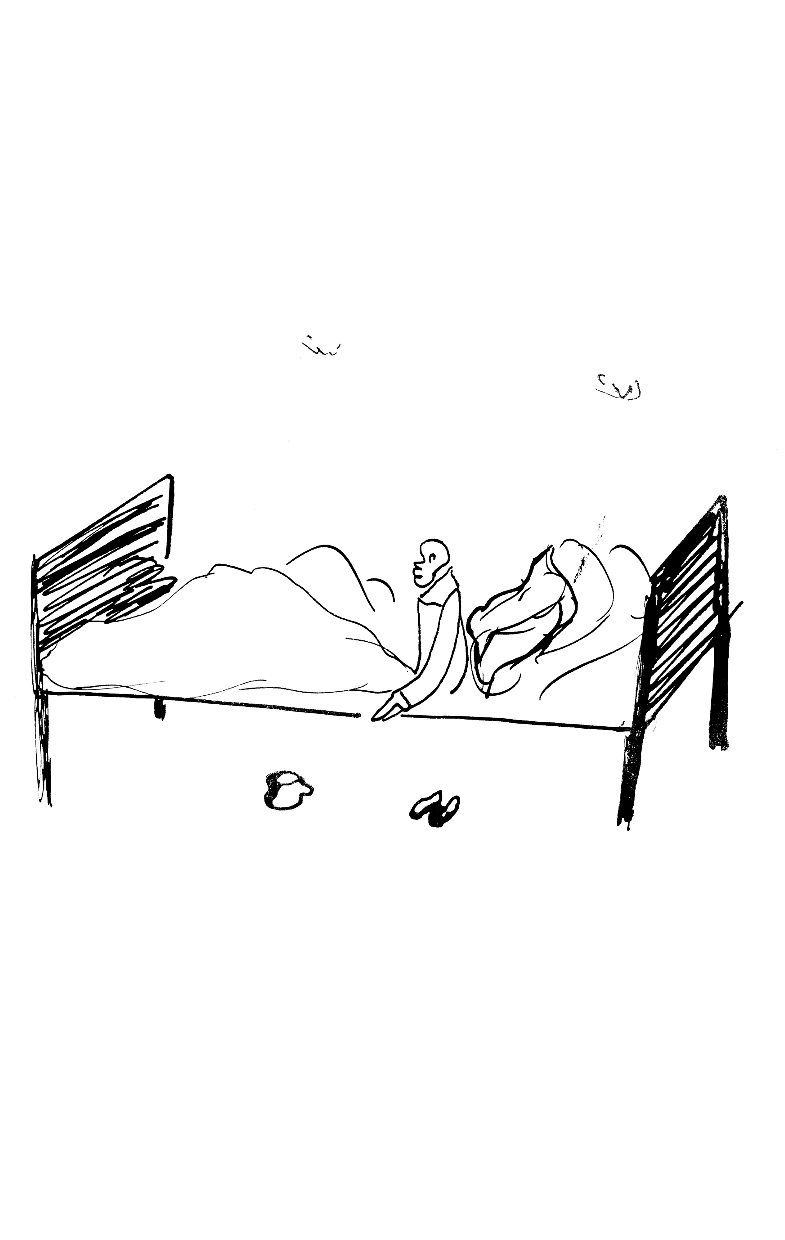
\includegraphics[width=\textwidth]{./IMAGENS/ESCOLHIDAS/IMG-03.pdf}
\end{figure}

“Gregor”, agora falava o pai, do cômodo à esquerda, “o senhor gerente veio
até aqui e quer saber por que você não partiu com o primeiro trem. Nós não
sabemos o que dizer a ele. E ele também quer falar com você em particular.
Então faça o favor de abrir a porta. Ele terá a bondade de desculpar a
desarrumação do quarto.” “Bom dia, senhor Samsa”, intrometeu-se o gerente,
chamando com voz amigável. “Ele não está bem”, a mãe disse ao gerente,
enquanto o pai ainda discursava para a porta, “ele não está bem, acredite,
senhor gerente. Se não, como Gregor iria perder um trem! O rapaz não tem
mais nada na cabeça a não ser a loja. Eu até fico irritada, porque ele
nunca sai à noite; agora mesmo, ele esteve oito dias seguidos na cidade,
mas ficou em casa todas as noites. Ele senta à mesa com a gente, e fica
quieto lendo o jornal ou estudando o horário dos trens. Já é uma grande
distração quando se ocupa com algum trabalho de marcenaria. Agora mesmo,
por exemplo, em duas ou três noites ele acabou de entalhar uma pequena
moldura; o senhor vai ficar admirado de ver como ela ficou bonita; está
pendurada lá dentro, no quarto; o senhor vai ver, assim que Gregor abrir.
Eu, aliás, fico contente que o senhor esteja aqui, senhor gerente; só a
gente não seria capaz de fazer o Gregor abrir a porta; ele é tão teimoso;
e com certeza não está nada bem, apesar de ter dito o contrário hoje de
manhã.” “Já vai”, disse Gregor, calculadamente lento, e não se mexeu, para
não perder nenhuma palavra da conversa. “De outro modo, prezada senhora,
eu também não saberia explicar”, disse o gerente, “tomara que não seja
nada sério. Embora, por outro lado, eu seja também obrigado a dizer que
nós, homens de negócios --- feliz ou infelizmente, como queira ---, muitas
vezes, em atenção às obrigações comerciais, devemos simplesmente ignorar
qualquer indisposição passageira.” “Então, o senhor gerente já pode
entrar?”, perguntou o pai com impaciência, e voltou a bater na porta.
“Não”, disse Gregor. No cômodo da esquerda sobreveio um silêncio
perturbador, no quarto da direita, a irmã começou a soluçar.

%\begin{figure}[htpb!

Por que será que a irmã não ia se juntar aos outros? Na certa só agora ela
havia saído da cama e ainda não se vestira. E por que chorava? Por que ele
não se levantava e não deixava o gerente entrar, por que se arriscava a
perder o emprego e por que desse jeito o chefe voltaria a perseguir os pais
com as antigas cobranças? Por enquanto, porém, essas eram preocupações de
todo desnecessárias. Gregor ainda estava presente e não tinha a menor
intenção de abandonar sua família. É certo que no momento ele continuava
lá, estendido no tapete, e ninguém que tivesse conhecimento de sua
situação iria lhe pedir a sério que deixasse o gerente entrar. Contudo,
por causa dessa pequena descortesia, para a qual mais tarde seria fácil
achar uma desculpa aceitável, Gregor não poderia ser mandado embora assim,
sumariamente. E lhe parecia muito mais lógico deixá-lo em paz
neste momento, em vez de perturbá-lo com choros e exortações. Mas era sem
dúvida a incerteza que afligia os outros e lhes desculpava o
comportamento.

“Senhor Samsa”, chamou então o gerente, em voz alta, “o que se passa? O
senhor fica entrincheirado aí em seu quarto, responde apenas com
monossílabos, deixa, sem necessidade, seus pais gravemente preocupados e ---
isso seja dito só de passagem --- falta às suas obrigações comerciais de uma
maneira realmente nunca vista. Eu falo aqui em nome de seus pais e do seu
chefe e lhe solicito, com toda a seriedade, o favor de uma explicação
clara e imediata. Estou atônito, estupefato. Eu acreditava conhecê-lo como
um homem pacato, ajuizado, e agora o senhor de repente dá mostras de
querer começar a exibir tais caprichos. É verdade que o chefe hoje de
manhã me insinuou uma possível explicação para a sua negligência --- dizia
respeito à cobrança recentemente confiada ao senhor ---, mas eu interpus a
bem da verdade quase a minha palavra de honra, dizendo que essa explicação
não tinha cabimento. Agora, contudo, que vejo sua obstinação
incompreensível, perco por completo a vontade de intervir o mínimo que
seja a seu favor. E sua posição não é em absoluto das mais garantidas. Eu
tinha a princípio a intenção de lhe dizer isso tudo em particular, porém,
já que o senhor me faz vir aqui desperdiçar inutilmente o meu tempo, não
sei por que também os seus pais não devam ouvir. Seus resultados nos
últimos tempos, aliás, não foram muito satisfatórios; claro que esta não é
a época do ano em que se fecham grandes negócios, nós reconhecemos; mas
uma época do ano em que não se fecha negócio algum, isso terminantemente
não existe, senhor Samsa, não pode existir.”

“Mas, senhor gerente”, Gregor gritou fora de si, esquecendo tudo o mais no
alvoroço, “eu abro agora mesmo, num instante. Um pequeno mal-estar, uma
tontura, impediu que eu me levantasse. Ainda estou aqui deitado. Mas já me
sinto mais disposto. Acabo mesmo de me levantar da cama. Só um minutinho
de paciência! Ainda não estou tão bem como pensava. Mas já me sinto
melhor. Como um homem pode ser pego assim de surpresa! Ainda ontem à noite
estava tudo bem comigo, meus pais são testemunha, ou melhor, já ontem à
noite eu tive um leve pressentimento. Deviam ter reparado em mim. Por que
não mandei logo avisar na loja?! Mas a gente sempre pensa que vai vencer a
doença sem precisar ficar em casa. Senhor gerente! Poupe os meus pais!
Todas as acusações que o senhor me faz agora, elas não têm fundamento;
também não me disseram uma palavra a esse respeito. Talvez o senhor não
tenha tomado conhecimento dos últimos pedidos que eu despachei. A
propósito, ainda saio para viajar com o trem das oito, essas poucas horas
de descanso me fortaleceram. Não é preciso se demorar mais, senhor
gerente; agora mesmo eu vou para a loja, e o senhor tenha a bondade de
transmitir esse recado e apresentar os meus cumprimentos ao senhor chefe.”

E enquanto Gregor despejava tudo isso às pressas, mal sabendo o que dizia,
havia se aproximado do guarda-roupa com facilidade, graças à prática
adquirida antes na cama, e procurava se levantar apoiado nele.
Queria muito abrir a porta, queria de fato mostrar-se e falar com o
gerente; estava ansioso para saber o que iriam dizer quando o vissem, eles
que agora tanto reclamavam sua presença. Se tomassem um susto, Gregor não
precisava justificar mais nada, e podia ficar descansado. E se aceitassem
tudo com calma, então também não havia motivo para se preocupar, e ele
poderia, se se apressasse, estar de fato às oito horas na estação
ferroviária. No começo ele escorregou algumas vezes no guarda-roupa liso,
mas ao final deu um último arranco e conseguiu se erguer; já não prestava
atenção à dor na parte de baixo de seu corpo, por mais que ardesse.
Deixou-se depois cair em direção ao encosto de uma cadeira próxima, a cujas
bordas se agarrou com suas perninhas. Só aí voltou a recuperar o domínio
sobre si mesmo e emudeceu, pois agora precisava ouvir o gerente.

“Os senhores entenderam uma única palavra?”, perguntou o gerente aos pais,
“não estará ele nos pregando uma peça?” “Meu Deus do céu”, exclamou a mãe
já começando a chorar, “ele pode estar muito doente, e nós aqui o
atormentando. Grete! Grete!”, gritou então. “Mamãe?”, respondeu a irmã do
outro lado. Elas se comunicavam através do quarto de Gregor. “Você tem que
chamar o médico agora mesmo. Gregor está doente. Corre até o médico. Você
ouviu como ele falou?” “Era uma voz de animal”, disse o gerente num tom
estranhamente baixo, em contraste com os gritos da mãe. “Anna! Anna!”,
chamou o pai batendo palmas da antessala para a cozinha, “vai já buscar um
chaveiro!” Logo as duas moças atravessavam a antessala correndo num frufru
de saias --- como é que a irmã havia se vestido tão rápido? --- e abriam
precipitadas a porta do apartamento. Não se ouviu a porta bater de volta;
decerto a tinham deixado aberta, como é de costume nas casas onde
aconteceu uma grande desgraça.

Gregor, porém, ficou bem mais tranquilo. É fato que suas palavras já não
eram compreendidas, embora tenham lhe parecido claras, mais claras até do
que antes, talvez porque seu ouvido logo se ajustara a elas. Mas, ainda
assim, agora já sabiam que nem tudo estava em ordem com ele, e se
dispunham a ajudá-lo. Fizeram-lhe bem a confiança e a firmeza com que as
primeiras providências foram tomadas. Ele se sentiu de novo integrado ao
círculo humano e esperava de ambos, médico e chaveiro, sem distingui-los
com muita precisão, realizações grandiosas e surpreendentes. A fim de
participar das discussões decisivas que estavam por vir com a voz o mais
clara possível, tossiu limpando a garganta, todavia se esforçou para
abafar o ruído, que provavelmente também teria um som distinto da tosse
humana, algo que ele mesmo já não tinha competência para discernir. No
cômodo do lado, nesse meio tempo, fez-se completo silêncio. Talvez os pais
tenham ido se sentar à mesa com o gerente, e cochichavam, talvez
estivessem todos pregados à porta, na escuta.

Gregor moveu-se até lá empurrando a cadeira devagar, depois soltou-a,
jogou-se contra a porta, segurou-se a ela mantendo-se na vertical --- as
pontas de suas perninhas tinham uma espécie de grude --- e descansou ali um
instante do esforço realizado. A seguir, contudo, foi tentar girar com a
boca a chave na fechadura. Era de lamentar que não tivesse uns dentinhos
de verdade --- com o que mais iria se agarrar à chave? ---, mas em compensação
as mandíbulas eram muito fortes, com certeza; com a ajuda delas de fato
conseguiu movimentar a chave e nem reparou que assim fatalmente infligia a
si mesmo algum ferimento, dado que um líquido marrom saía-lhe da boca,
escorria pela chave e pingava no chão. “Prestem atenção”, disse o gerente
no cômodo ao lado, “ele está virando a chave.” Para Gregor, esse foi um
grande incentivo; mas todos deveriam apoiá-lo, inclusive o pai e a mãe:
“Ânimo, Gregor”, deveriam gritar, “não desiste, dá duro na fechadura!”
Então, imaginando que todos acompanhavam seus esforços com interesse,
aferrou-se à chave sem pensar em mais nada, reunindo todas as forças que
podia. Bailava em torno da fechadura conforme o avanço da volta da chave;
acabou segurando-se na vertical apenas com a boca, e de acordo com a
necessidade pendurava-se na chave ou a forçava mais uma vez para baixo com
todo o peso do seu corpo. O claro estalo da fechadura que enfim destravava
tirou-o do transe. Tomando fôlego, ele disse: “Pois então, nem precisei do
chaveiro”, e deitou a cabeça na maçaneta, para abrir de par em par as
folhas da porta.

Como só podia abri-las puxando daquela maneira, uma delas já estava
praticamente toda aberta e ele mesmo ainda não podia ser visto. Devia
primeiro contornar devagar essa folha, e sempre com muita cautela, se não
quisesse fazer o papelão de cair de costas bem na entrada do quarto.
Estava ainda ocupado com essa difícil operação e não tinha tempo para
prestar atenção em outra coisa, quando ouviu o gerente soltar um sonoro
“Oh!” --- soava como o sopro do vento --- e então Gregor o enxergou também,
viu como ele, que era o que estava mais próximo da porta, comprimia com a
mão a boca aberta e retrocedia aos poucos, parecia puxado por uma força de
atração contínua, invisível. A mãe --- que apesar da presença do gerente
apresentava-se com os cabelos ainda soltos, desgrenhados pela noite de
sono --- juntou as mãos e olhou primeiro para o pai, depois deu dois passos
na direção de Gregor e despencou no meio do círculo formado por suas saias
esparramadas, o rosto encoberto pendendo contra o peito. O pai cerrou o
punho com uma expressão ameaçadora, como se quisesse forçar Gregor a
voltar para dentro do quarto, então olhou a sala em torno de si, indeciso,
cobriu os olhos com as mãos e caiu num choro que chegou a sacudir seu
peito forte.

Gregor contudo não havia nem saído do quarto, ainda se esticava de dentro
na direção da folha que permanecia trancada, de modo que se avistavam
apenas metade de seu corpo e acima, inclinada para o lado, a cabeça com a
qual olhava de soslaio para os outros. Havia clareado bastante nesse meio
tempo; no outro lado da rua projetava-se nítido um recorte do imenso
edifício da frente, cinza escuro --- era um hospital ---, com suas janelas
rigorosamente simétricas rasgando a fachada; a chuva ainda caía, mas eram
apenas gotas grossas, esparsas, e que assim espaçadas atingiam o solo num
ritmo regular. A louça do café espalhava-se em grande número sobre a mesa,
pois para o pai o café da manhã era a refeição mais importante do dia, e
ele a prolongava horas a fio com a leitura de diferentes jornais. Na
parede oposta pendia uma fotografia de Gregor da época do exército,
posando como tenente, as mãos na espada, sorrindo despreocupado, invocando
respeito por sua postura e sua farda. A porta da antessala estava aberta
e, como a porta da frente também continuava aberta, era possível enxergar
na parte de fora o corredor e o começo das escadas que conduziam para
baixo.

“Bem”, disse Gregor, com a plena consciência de que era o único que havia
mantido a calma, “agora mesmo vou me vestir, empacotar as amostras e
partir. Vocês vão querer, por favor, me deixar partir? Como vê, senhor
gerente, não estou sendo teimoso e trabalho com vontade; as viagens são
incômodas, mas eu não poderia viver sem viajar. Para onde está indo,
senhor gerente? Para a loja? É? O senhor vai reportar tudo direitinho? Uma
pessoa pode estar num momento incapacitada para o trabalho, mas essa é
exatamente a hora certa de recordar suas realizações passadas e de pensar
que depois, afastado o impedimento, com certeza ela virá a trabalhar até
mesmo com mais aplicação e concentração do que antes. O senhor sabe muito
bem o tanto que eu devo ao chefe. E ainda tenho de cuidar dos meus pais e
da minha irmã. Estou na penúria, mas com o trabalho vou conseguir dar a
volta por cima. Não torne as coisas mais difíceis do que já são para mim.
Tome o meu partido na loja! Eu sei que ninguém gosta do caixeiro-viajante.
Pensam que ele ganha rios de dinheiro e além disso leva uma vida folgada.
Ninguém nem mesmo toma a iniciativa de discutir mais a fundo esse
preconceito. Mas o senhor, senhor gerente, tem uma visão geral da situação
melhor que a dos outros empregados, até mesmo, seja dito em absoluto
segredo, melhor que a do próprio chefe, que em sua posição de patrão às
vezes se deixa levar por juízos equivocados, prejudicando um funcionário.
O senhor também sabe muito bem que o caixeiro-viajante, que passa quase o
ano inteiro fora da loja, torna-se facilmente vítima de intrigas,
maledicências e queixas infundadas, das quais é impossível que se defenda,
porque na maioria das vezes ele nem chega a tomar conhecimento delas e é só
quando volta para casa, esgotado após outra viagem, que vem a receber de
corpo presente suas graves consequências, cujas causas originais não tem
mais como descobrir. Senhor gerente, não vá embora sem me dizer uma
palavra demonstrando que ao menos em parte o senhor me dá alguma razão!”

Mas o gerente, logo às primeiras palavras, já havia lhe dado as costas e,
com um esgar de lábios, só ousava olhar em sua direção por cima dos ombros
trêmulos. E durante o discurso de Gregor não permaneceu parado um segundo
sequer, ao contrário, sem perdê-lo de vista, retrocedeu em direção à
porta, porém muito devagar, como se houvesse uma lei misteriosa que o
proibisse de deixar a sala. Aos poucos chegou à antessala e, a julgar pelo
movimento repentino com que retirou o pé no último passo para fora da
sala, era possível acreditar que tivesse pisado em brasas. Já na
antessala ele esticava a mão direita cada vez mais na direção da escada,
como se lá o aguardasse uma salvação decididamente extraterrena.

Gregor sabia que em hipótese alguma devia deixar o gerente partir naquele
estado de espírito, se não quisesse que sua posição na loja ficasse
comprometida. Os pais não entendiam direito o que acontecia; ao longo dos
anos, haviam formado a convicção de que Gregor estava garantido na loja
até o fim da vida, e agora, ainda por cima, com a urgência da situação,
tinham tanto a fazer que uma conjetura dessas lhes passava despercebida.
Mas a Gregor não passava. Era preciso reter o gerente, apaziguá-lo,
persuadi-lo e por fim convencê-lo; o futuro de Gregor e de sua família
dependia muito disso! Quem dera a irmã estivesse aqui! Ela era
inteligente; chorou por antecipação quando Gregor ainda estava só deitado
quieto, virado de costas. E na certa o gerente, esse conquistador, iria se
deixar levar por ela; que fecharia a porta do apartamento e ali mesmo na
antessala o acalmaria. Mas a irmã nem ao menos estava lá, Gregor mesmo
devia cuidar do assunto. E sem pensar que nada sabia de sua real
capacidade de se movimentar, sem pensar também que era possível, ou
melhor, muito provável que seu discurso mais uma vez não houvesse sido
compreendido, ele largou a folha da porta e se lançou pela abertura;
queria correr para junto do gerente que, de um modo patético, já se
agarrava com ambas as mãos ao corrimão do corredor; porém, no instante
seguinte, procurando algum apoio, Gregor deu um gritinho e caiu por cima
de suas perninhas. Mal isso aconteceu, ele experimentou, pela primeira vez
naquela manhã, algum conforto físico; as perninhas encontraram chão firme
abaixo de si; e obedeciam de pronto, como ele notou com satisfação; até
faziam força para levá-lo aonde quisesse; e ele logo acreditou que era
iminente a melhora definitiva de todos aqueles incômodos. Porém, no mesmo
momento em que se viu ali no chão, agitado pelo desejo de se movimentar,
não muito afastado de sua mãe, justamente à sua frente, ela, que parecia
tão recolhida dentro de si mesma, de um pulo se levantou, os braços
esticados, apontava com o dedo, gritando: “Socorro, meu Deus do céu,
socorro!”, mantinha a cabeça inclinada, como se quisesse observar Gregor
com mais atenção, entretanto, num gesto contraditório, recuava sem pensar em
mais nada; esquecera que atrás de si a mesa estava posta; quando encostou
nela, como que distraída, sentou-se logo sobre o tampo; e pareceu nem
reparar que a seu lado, saindo do grande bule que virara, o café derramava
em grandes golfadas sobre o tapete.

\begin{figure}[p]
\centering
\thisfloatpagestyle{empty}
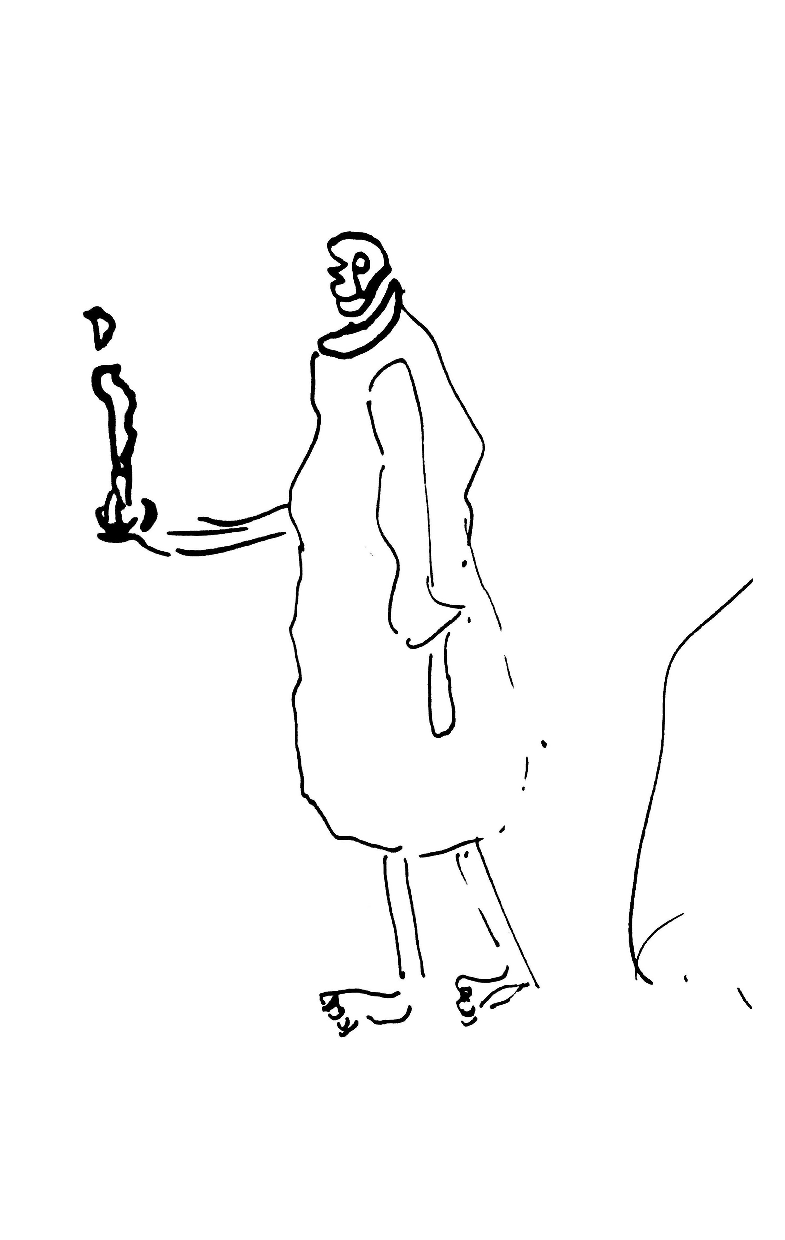
\includegraphics[width=\textwidth]{./IMAGENS/ESCOLHIDAS/IMG-05.pdf}
\end{figure}

“Minha mãe”, Gregor disse baixinho, e olhou na direção dela. Por um
instante, o gerente foi varrido de seus pensamentos; em contrapartida,
ante a visão do café que escorria, não pôde deixar de estalar várias vezes
as mandíbulas, com cobiça. Diante disso, a mãe soltou um novo grito, saiu
correndo da mesa e caiu nos braços do pai, que veio depressa ao seu
encontro. Gregor, contudo, agora não tinha tempo para os pais; o gerente
já descia a escada; o queixo na altura do corrimão, ainda voltava o olhar
pela última vez. Gregor se preparou para correr, na expectativa de alcançá-lo;
o gerente deve ter pressentido alguma coisa, pois de um salto desceu
vários degraus e desapareceu; mas ainda soltou um grito, “Ahh!”, que ecoou
em toda a escadaria. Por infelicidade, então, parece que a evasão do
gerente também deixou o pai, que até aqui havia se comportado de modo
relativamente calmo, bastante transtornado, pois, em vez de
correr ele mesmo atrás do homem ou de pelo menos permitir que Gregor saísse em seu
encalço, agarrou com a mão direita a bengala do gerente, por este deixada
na cadeira, junto com o chapéu e o sobretudo, apanhou com a mão esquerda
um grosso jornal de cima da mesa e, com passadas pesadas, sacudindo a
bengala e o jornal, pôs-se a tocar Gregor de volta para o quarto. Nenhuma
súplica lhe foi de valia, nenhuma súplica sequer fora entendida, Gregor
quis baixar a cabeça de modo ainda mais humilde, e o pai só fez bater os
pés com mais força ainda. Do lado oposto, a mãe, apesar do tempo frio,
havia aberto uma janela e, debruçada o mais para fora possível, apertava o
rosto contra as mãos. Da viela, pela escadaria, veio uma forte corrente de
ar, as cortinas esvoaçaram, os jornais farfalharam sobre a mesa, algumas
folhas voaram e foram parar no chão. Implacável, o pai insistia e passou a
silvar como um selvagem. Mas Gregor ainda não tinha a menor prática em
andar para trás, e ia realmente muito devagar. Se ao menos pudesse dar
meia volta, na mesma hora estaria dentro do quarto, mas ele temia
impacientar o pai com uma manobra muito demorada, e a todo instante via-se
ameaçado pelo golpe fatal da bengala, desferido em suas costas ou na
cabeça. Porém, no fim não restou nenhuma outra alternativa, pois ele notou
assustado que, ao andar para trás, nem uma vez sequer conseguira manter a
direção; e assim, entre olhadelas furtivas, medrosas e incessantes na
direção do pai, começou a se virar, o mais rápido que podia, na
verdade, contudo, ainda muitíssimo lento. Talvez o pai tenha notado a sua boa
vontade, porque não o atrapalhou nessa hora, pelo contrário, até
direcionou a volta aqui e ali, de longe, com a ponta da bengala. Se não
fossem aqueles silvos insuportáveis! Por causa deles, Gregor perdia a
cabeça. Já havia dado quase toda a volta quando, atordoado por aqueles
ruídos incessantes, chegou a se enganar e recuou um bom pedaço no sentido
contrário. Mas quando afinal, contente, viu-se diante da abertura da
porta, percebeu que seu corpo era muito largo para passar por ela sem
dificuldades. Ao pai, é lógico, naquele estado de ânimo, não ocorria nem
de longe abrir um pouco a outra folha da porta, de modo a deixar espaço
suficiente para a passagem de Gregor. Sua ideia fixa resumia-se a fazê-lo
entrar no quarto o mais rápido possível. Jamais toleraria também os
preparativos minuciosos de que precisava para se erguer e desse modo
tentar passar pela porta. Em vez de ajudar, agora fazendo um barulho infernal,
forçava o avanço de Gregor como se não houvesse nenhum obstáculo; soava
como se já não fosse mais a voz de um único pai apenas; com efeito, a
coisa deixou de ser brincadeira, e Gregor --- seja lá o que acontecesse ---
jogou-se contra a porta. Um dos lados de seu corpo subiu, ele ficou
atravessado na abertura, uma parte de suas costas foi toda esfolada, na
tinta branca da porta restaram manchas repulsivas, logo se viu prensado e
sozinho não teria podido mais se mexer, as perninhas do lado de cima
pendiam vibrando no ar, as do outro lado eram dolorosamente pressionadas
contra o chão --- foi quando o pai, de trás, deu-lhe um empurrão forte,
desta vez deveras libertador, e ele, sangrando a valer, entrou voando para
dentro do quarto. A porta ainda foi fechada com a bengala e então enfim
tudo ficou quieto. 

\chapter*{}
\openany
\section{II}

\noindent{}Só ao crepúsculo Gregor acordou de seu sono pesado, que mais parecia um
desmaio. Com certeza, se não fosse perturbado, também não teria acordado
muito mais tarde, pois sentia que já dormira e descansara o suficiente,
embora tivesse a impressão de haver sido despertado por alguns passos
furtivos e pelo ruído da porta de acesso à antessala, que fora trancada
por precaução. A fraca luz das lâmpadas elétricas da rua iluminava
palidamente alguns pedaços do teto do quarto e a parte de cima dos móveis,
mas Gregor embaixo estava às escuras. Aos poucos, tateando ainda
desajeitado com suas antenas, às quais só agora dava o devido valor,
deslocou-se até a porta, para ver o que havia ocorrido. Seu lado esquerdo
estava que era uma única cicatriz, comprida, esticada, incômoda, e por
isso ele tinha de andar mancando mesmo com suas duas fileiras de pernas.
Uma perninha, aliás, saíra seriamente machucada dos incidentes da manhã ---
era um milagre que apenas uma tivesse se machucado --- e pendia inerte,
arrastada pelas outras.

Só ao se aproximar da porta é que foi perceber o que o atraíra na verdade;
era o cheiro de alguma coisa comestível. Com efeito, lá estava uma tigela
cheia de leite fresco, no qual algumas migalhas de pão boiavam. Por pouco
não riu de tanta alegria, pois continuava com uma fome ainda maior do que
estava pela manhã, e na mesma hora mergulhou a cabeça no leite, quase até
os olhos. No instante seguinte porém a retirou, desapontado; não apenas
comer lhe era dificultoso, por causa do lado esquerdo avariado --- e ele só
podia comer com a colaboração ofegante de todo o corpo ---, mas também
acima de tudo não lhe apeteceu em absoluto o leite, que antes era sua
bebida favorita, e na certa por isso a irmã lho trouxera, de modo que ele,
meio enojado, deixou de lado a tigela, voltando a se arrastar para o
centro do quarto.

Na sala, como Gregor via pelas frinchas da porta, o gás fora aceso, porém,
enquanto antigamente a essa hora o pai se dedicava à leitura em voz alta
do jornal vespertino, para a mãe e à vezes também para a irmã, agora não
se ouvia ruído algum. Pode ser que essa leitura, que a irmã sempre lhe
descrevia e comentava nas cartas, tivesse saído da rotina nos últimos
tempos. Em todo caso, o silêncio prevalecia, embora com toda a certeza o
apartamento não estivesse vazio. “Mas que vida mais tranquila a família
leva”, disse Gregor com seus botões e, enquanto olhava fixo a escuridão à
sua frente, sentiu um grande orgulho de que pudesse proporcionar a seus
pais e a sua irmã uma vida dessas em um apartamento tão bom. Mas e se
agora todo o sossego, todo o bem-estar, toda a paz tivessem de chegar a um
terrível fim? Para não se perder em tais pensamentos, Gregor preferiu se
movimentar, e ficou se arrastando no quarto, de um lado para o outro.\looseness=-1

Durante a longa noite, as duas portas laterais, primeiro uma, depois a
outra, foram abertas uma frestinha apenas, e fechadas rapidamente em
seguida; alguém sem dúvida sentia necessidade de entrar, mas resolvera
pensar duas vezes. Gregor se deteve então bem na frente da porta da sala,
determinado a trazer a indecisa visita para dentro de alguma maneira, ou
pelo menos disposto a descobrir quem era; a porta porém não voltou a ser
aberta e ele esperou em vão. De manhã, quando as portas estavam trancadas,
todos queriam entrar, agora, depois que ele abrira sozinho uma delas, e as
outras ao que tudo indicava teriam sido abertas no decorrer do dia,
ninguém mais vinha, mesmo com as chaves do lado de fora.

Só bem tarde da noite é que desligaram a luz da sala, e nesse momento foi
fácil comprovar que os pais e a irmã haviam ficado acordados até aquela
hora, pois dava para ouvir direitinho como todos os três se afastavam na
ponta dos pés. Na certa até amanhã ninguém mais viria à procura de Gregor;
ele tinha assim bastante tempo para refletir, sem ser incomodado, sobre o
modo como devia reorganizar sua vida a partir de agora. Contudo, o quarto
alto e despojado, no qual era forçado a permanecer deitado contra o rés do
chão, angustiava-o, e ele não conseguia descobrir por que, uma vez que era
o mesmo quarto que habitava havia já cinco anos --- então, com uma meia
volta quase involuntária, e não sem certa vergonha, correu para debaixo do
canapé, onde se sentiu muito bem acomodado, apesar de suas costas meio
espremidas e apesar de não poder mais erguer a cabeça, lamentando apenas
que seu corpo fosse tão largo que não coubesse inteiro embaixo do móvel.\looseness=-1

Ali ele passou toda a noite, uma parte em cochilos dos quais era seguidas
vezes despertado de súbito pela fome, uma parte tomado por preocupações
e incertas esperanças de que tudo afinal encontraria uma solução, de que o
certo seria agir com calma nesse meio tempo e, com paciência e o máximo de
respeito aos familiares, tentar tornar suportável o desgosto que ele, em
suas atuais circunstâncias, excepcionalmente era obrigado a lhes causar.\looseness=-1

Já de manhã bem cedo, madrugadinha ainda, Gregor teve oportunidade de pôr
à prova suas ponderadas decisões, pois vindo da antessala a irmã, vestida
quase dos pés à cabeça, abriu a porta e examinou o interior do quarto com
apreensão. Ela não o descobriu na hora, mas quando o divisou ali embaixo
do canapé --- Deus do céu, ele tinha de estar em algum lugar, não podia sair
voando por aí --- levou um susto tão grande que, sem que pudesse se
controlar, voltou a fechar a porta no mesmo instante. Porém, parecendo
arrependida de sua atitude, tornou a abri-la em seguida e entrou na ponta
dos pés, como se ali estivesse alguém muito doente ou fosse um estranho.
Gregor estendeu um tantinho a cabeça até a borda do canapé e observou a
irmã. Iria ela notar que ele tinha deixado o leite intacto, lógico que de
modo algum por falta de apetite, e será que traria uma outra comida que
lhe fosse mais adequada? Se ela não tomasse a iniciativa, ele preferia
morrer de fome a ter de chamar sua atenção para isso, embora no fundo
sentisse uma vontade urgente de deixar o canapé, se atirar aos pés da irmã
e pedir a ela algo de bom para comer. Mas a irmã, surpresa, logo notou a
tigela ainda cheia, ao redor da qual havia apenas um pouco de leite
derramado, recolheu-a no mesmo instante, claro que não com as mãos nuas, e
sim com um pedaço de pano, e a levou para fora. Gregor ficou bastante
curioso para saber o que ela traria em troca, e teceu as mais diversas
suposições a respeito. Nunca, porém, teria adivinhado o que a irmã, em sua
grande bondade, realmente fez. A fim de testar o seu paladar, ela lhe
trouxe várias coisas sortidas, que dispôs em uma folha de jornal velho.
Havia ali legumes passados já meio apodrecidos; ossos da última ceia
recobertos de molho branco ressecado; uma porção de passas e amêndoas; um
queijo que há dois dias Gregor julgara intragável; um pedaço de pão duro,
uma fatia de pão com manteiga e outra fatia com manteiga e sal. Além
disso, à frente de tudo voltou a colocar a tigela, pelo visto destinada de
uma vez por todas a ele, agora cheia de água. E por delicadeza, sabendo
que Gregor não iria comer diante dela, afastou-se às pressas e chegou a
dar a volta na chave, a fim de que ele notasse que poderia se pôr tão à
vontade quanto quisesse. As perninhas de Gregor zuniram quando ele partiu
na direção da comida. Suas feridas, aliás, já deviam ter sarado de todo,
ele não sentia mais nenhum desconforto, o que o deixou pasmo pois lembrou
como, mais de um mês atrás, havia feito com a faca um cortinho de nada no
dedo, e esse machucado ainda antes de ontem doía um bocado. “Será que
minha sensibilidade diminuiu?”, pensou, e sorveu ávido o queijo, que acima
de todas as outras comidas o atraíra imediata e energicamente. Com
rapidez, um após o outro, vertendo lágrimas de contentamento, ele devorou
o queijo, os legumes e o molho; os alimentos frescos, ao contrário, não
agradavam o seu paladar, ele mal podia suportar-lhes o cheiro, e teve até
de afastar para o lado as coisas que queria comer. Já dera cabo de tudo há
algum tempo, e continuava largado no mesmo lugar, apenas descansando,
quando a irmã, para sinalizar que ele devia retroceder, deu uma volta na
chave. Isso o despertou de pronto, quando estava a ponto de cochilar, e
ele voltou correndo para debaixo do canapé. Mas precisou de muito
autocontrole para permanecer ali embaixo durante o curto espaço de tempo
em que a irmã esteve no quarto, porque, após a lauta refeição, seu corpo
ficou mais redondo e ele mal conseguia respirar naquele aperto. Entre
breves crises de asfixia, viu com os olhos um pouco saltados a irmã, sem
desconfiar de nada, juntar com uma vassoura não apenas as sobras, mas
inclusive os alimentos em que ele nem sequer chegara a tocar, como se
esses também não pudessem mais ser aproveitados, e a viu ainda despejar
tudo depressa em um balde que cobriu com uma tampa de madeira e levou para
fora do quarto. Mal ela lhe deu as costas, Gregor avançou logo para fora
do canapé e relaxou, voltando a estufar-se.

Dessa maneira recebia doravante Gregor diariamente sua refeição, a
primeira vez de manhã, quando os pais e a empregada ainda dormiam, a
segunda vez depois que todos almoçavam, pois era o momento em que os dois
dormiam de novo ainda um bocadinho, e a empregada saía, encarregada pela
irmã de uma incumbência qualquer. Com certeza os pais não queriam que
Gregor morresse de fome, porém talvez só suportassem, da experiência de
suas refeições, no máximo ouvir dizer que aconteciam, ou quem sabe a irmã
quisesse lhes poupar mais uma aflição, ainda que pequena, pois era visto
que já sofriam o bastante.\looseness=-1

\textls[-10]{Gregor não chegou a saber com quais desculpas o médico e o chaveiro foram
dispensados naquela manhã inicial, porque, como não o compreendiam,
ninguém presumia, nem mesmo a irmã, que ele pudesse compreender os outros,
e por isso, quando ela estava no quarto, ele era obrigado a se contentar
apenas com os suspiros e os lamentos que de vez em quando escutava. Só
depois que ela se acostumou um pouco com tudo --- uma aceitação completa,
claro, não poderia nunca ser cogitada ---, é que Gregor chegou a flagrar
algumas vezes uma observação mais simpática ou que assim poderia ser
entendida. “Acho que hoje estava bom”, ela falava, quando Gregor havia
devorado com gosto a refeição, ou, caso contrário, o que gradativamente
foi se repetindo com maior frequência, costumava dizer, meio entristecida:
“De novo não tocou em nada”.}\looseness=-1

Mas, conquanto não conseguisse saber de nenhuma novidade diretamente,
Gregor captava quase tudo o que vinha dos cômodos adjacentes, e assim que
escutava alguma voz corria no ato até a porta respectiva e colava-se a ela
com o corpo todo. Sobretudo nos primeiros tempos, não havia uma conversa
que, de algum modo, ainda que só às escondidas, não tratasse dele. Dois
dias seguidos, durante todas as refeições, só se ouviram deliberações
sobre como deviam se comportar daí em diante; mas também entre as
refeições falava-se do mesmo assunto, pois havia sempre no mínimo dois
membros da família em casa, dado que ninguém queria ficar sozinho ali e
não tinham a menor condição de abandonar o apartamento logo de uma vez.
Ainda nos primeiros dias --- não estava muito claro nem o que nem o quanto
ela sabia do incidente --- a empregada pediu de joelhos à mãe que a mandasse
embora de imediato, e quando, quinze minutos depois, deixava o emprego,
agradeceu com lágrimas nos olhos tanto a demissão quanto o imenso favor
que nessa hora lhe prestavam, e jurou de pé junto, sem que isso lhe fosse
solicitado, não revelar o menor detalhe a ninguém.\looseness=-1

\begin{figure}[p]
\centering
\thisfloatpagestyle{empty}
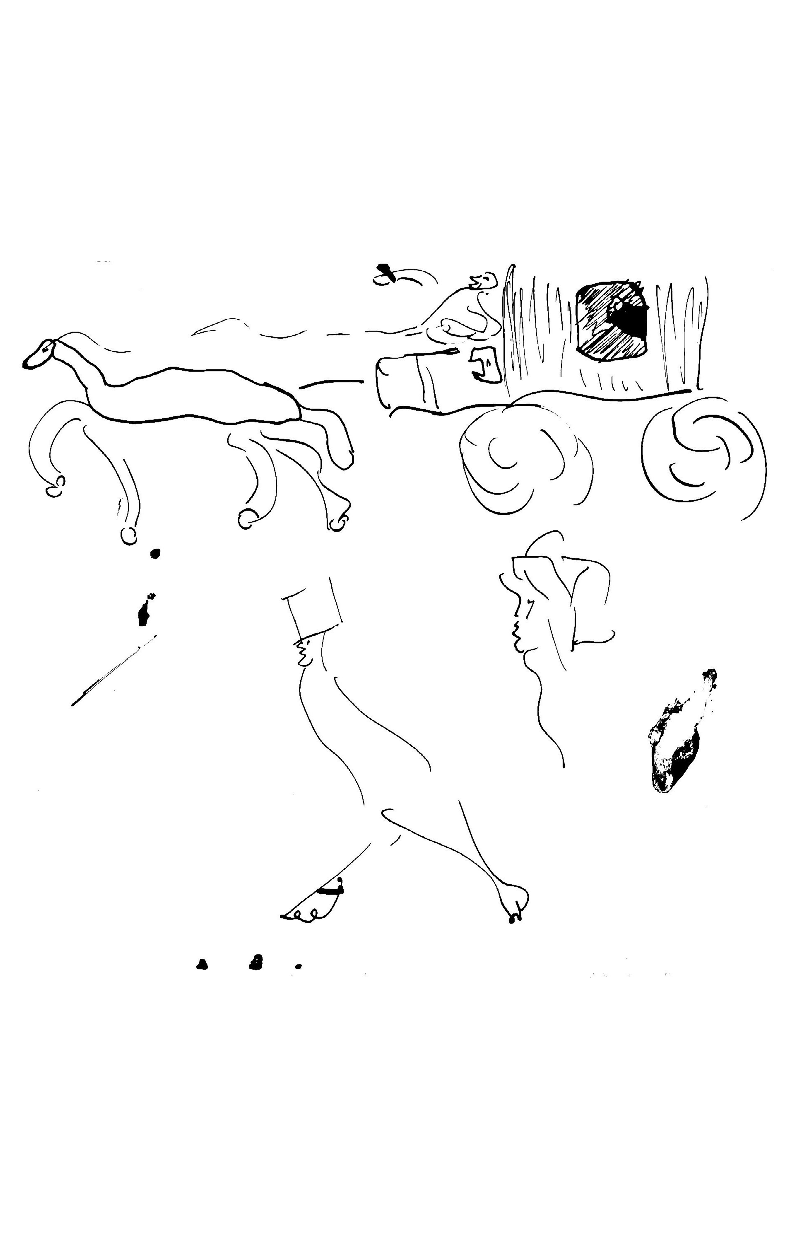
\includegraphics[width=\textwidth]{./IMAGENS/ESCOLHIDAS/IMG-06.pdf}
\end{figure}

Então a irmã se viu também obrigada a ajudar a mãe na cozinha; em todo
caso, não era muito o esforço exigido, pois não se comia quase nada.
Gregor ouvia vezes seguidas como um deles incentivava em vão o outro a
comer, sempre obtendo como única resposta: “Obrigado, estou satisfeito”,
ou algo semelhante. Tampouco deviam beber. Em várias ocasiões a irmã
perguntava ao pai se ele não queria cerveja, e se punha com alegria à
disposição para ela mesma ir buscar ou então, ante o silêncio do pai e
para eliminar qualquer suspeita de inconveniência, dizia que podia mandar
a zeladora ir no lugar dela, mas daí o pai respondia com um poderoso “Não”
final, e não se falava mais no assunto.

Já no decorrer desses primeiros dias o pai expôs a ambas, mãe e irmã, suas
reais perspectivas e condições financeiras. Aqui e ali ele deixava a mesa
para ir buscar algum comprovante ou alguma caderneta no pequeno e valioso
cofre que conseguira salvar da bancarrota de seu negócio, ocorrida há
cinco anos. Ouvia-se ele destravar a complicada fechadura e, depois de
retirar o que buscava, voltar a trancá-la. Essas explicações do pai, por
um lado, foram as primeiras boas notícias que Gregor chegou a ouvir desde
o seu confinamento. Sempre achara que nada havia sobrado para o pai do
antigo negócio, pelo menos o pai nunca lhe dissera o contrário, e de
qualquer modo Gregor também nunca lhe perguntara nada a respeito. Sua
única preocupação na época havia sido fazer de tudo para que a família
superasse o mais rápido possível o contratempo comercial, que deixara
todos no mais completo desalento. E foi assim que ele começou a trabalhar
com uma disposição fora do comum, e passou da noite para o dia de simples
balconista a caixeiro-viajante, função que evidentemente lhe abria muitas
outras oportunidades de ganho, e cujos ótimos resultados, sob a forma de
comissões, rápido se transformaram em dinheiro vivo que podia ser
espalhado sobre a mesa em casa, diante da família assombrada e satisfeita.
Foram bons tempos aqueles, que depois nunca mais se repetiram, pelo menos
não com igual esplendor, apesar de Gregor ter recebido mais tarde ainda
muito dinheiro, o que o capacitava a assumir, como assumiu, as despesas de
toda a família. Tanto a família quanto Gregor se acostumaram logo a essa
situação, eles aceitavam o dinheiro agradecidos, ele o entregava de bom
grado, mas não houve mais nenhuma manifestação efusiva. Só a irmã
permaneceu próxima a Gregor, ela que diferente dele amava a música e
aprendera a tocar violino de um modo enternecedor, e ele planejava em
segredo matriculá-la no conservatório no próximo ano, sem ligar para os
altos custos que isso devia acarretar, e que seriam compensados de uma ou
outra maneira. Várias vezes, nas conversas com a irmã, durante as curtas
estadias de Gregor na cidade, o conservatório era mencionado, porém sempre
como se fosse apenas um belo sonho, cuja realização era impensável, e os
pais não ouviam essas fantasias inocentes com muita satisfação; mas Gregor
havia refletido a sério sobre o assunto e pretendia anunciar seus planos
oficialmente na noite de Natal.

Esses pensamentos, inúteis na sua situação atual, passavam-lhe pela cabeça
enquanto permanecia lá erguido e colado à porta, escutando. Às vezes,
devido ao cansaço de todo o corpo, não conseguia mais prestar atenção e
deixava sem querer a cabeça bater na porta, mas a endireitava no mesmo
instante, pois até o mínimo ruído que dessa forma provocava era ouvido do
lado de fora e fazia todos se calarem. “Que será que tanto se mexe”, dizia
o pai momentos depois, a voz alta dirigida para a porta, e só aos poucos a
conversa interrompida era retomada.

Gregor ficou então cansado de saber --- pois o pai fazia questão de repetir
sucessivas vezes suas explicações, em parte porque há muito que ele
próprio já não se ocupava dessas coisas, em parte também porque a mãe não
compreendia tudo logo na primeira vez --- que apesar de toda a desgraça
ainda tinham disponível uma sobra orçamentária dos velhos tempos, em todo
caso bastante pequena, mas que nesse ínterim os juros acumulados haviam
feito crescer um pouquinho. Além disso também havia o dinheiro que Gregor
todo mês deixava em casa --- retirava para si apenas algumas notas ---, que
não era integralmente gasto e acumulara-se, originando um pequeno capital.
Atrás da porta, Gregor balançou a cabeça em sinal de aprovação, contente
com essa inesperada prudência e economia. Era bem verdade que, com esse
excedente de dinheiro, já poderia ter quitado outras parcelas da dívida
que o pai tinha com o chefe, e aquele dia em que poderia enfim se libertar
do emprego já estaria mais próximo, porém agora sem dúvida as coisas
estavam melhor assim, do jeito que o pai havia organizado.

Contudo, a quantia não era em absoluto suficiente para que se pudesse
viver de seus rendimentos; talvez bastasse para manter a família durante
um, no máximo dois anos, para mais não dava. Eram portanto apenas
economias de que não podiam dispor, e deviam conservar intactas para um
caso de maior necessidade; o dinheiro do dia-a-dia teria de ser ganho.
Acontece, no entanto, que o pai, embora ainda com saúde, era um homem
idoso, que estava há cinco anos totalmente afastado do trabalho e além do
mais já não podia fazer muito esforço; nesses cinco anos, que foram as
primeiras férias de sua vida diligente porém malsucedida, ele engordara
muito e por causa disso havia ficado mole e pesadão. E devia a velha mãe,
porventura, ir atrás do dinheiro, ela que sofria de asma e ficava cansada
só de andar pelo apartamento e que, dia sim dia não, passava deitada no
sofá, de janelas abertas, com crises respiratórias? Ou iria conseguir
dinheiro a irmã, ainda uma criança com seus dezessete anos e que até o
momento tivera uma vida invejável, nada mais que cuidar de se vestir,
dormir até tarde, ajudar um pouco na casa, uma ou outra atividade de lazer
modesta e tocar violino acima de tudo? Sempre que a conversa chegava na
necessidade de ganhar dinheiro, Gregor primeiro se soltava e em seguida se
jogava sobre o frio sofá de couro encostado ao lado da porta, pois ficava
inflamado diante de tanta humilhação e infortúnio.

Era frequente ele passar a noite inteira ali em cima, sem dormir um só
minuto, horas seguidas apenas arranhando o couro. Salvo quando se dispunha
a encarar o grande esforço de empurrar uma cadeira até a janela, depois
subir rastejando até alcançar o parapeito e, apoiado na cadeira,
inclinar-se para frente, óbvio que apenas como uma espécie de recordação
da sensação de liberdade que antes tinha ao olhar pela janela. Pois era
patente que dia após dia via cada vez com menos nitidez as coisas que
estavam afastadas de si; não avistava mais o hospital do outro lado, cuja
visão cotidiana obrigatória ele antes amaldiçoava, e, se não tivesse
certeza absoluta de que morava na travessa Charlotte, uma viela tranquila,
não obstante sua total urbanidade, seria capaz de acreditar que sua janela
dava para um deserto no qual o cinza do céu e o cinza da terra se juntavam
e eram indistinguíveis. Bastou à atenciosa irmã ver em duas ocasiões a
cadeira encostada na janela para que todas as vezes, depois de arrumar o
quarto, voltasse a colocá-la no mesmo lugar, e a partir de então até a
folha interna da janela era deixada aberta.

Se Gregor pudesse falar com a irmã, e agradecê-la por tudo que estava
obrigada a fazer por ele, aceitaria os favores com mais facilidade; assim,
porém, ele sofria. A irmã decerto procurava disfarçar ao máximo o que
havia de penoso em tudo aquilo e, é claro, quanto mais o tempo passava,
tanto melhor ela o conseguia, entretanto, com o passar do tempo também
Gregor veio a perceber as coisas com maior exatidão. A entrada dela já lhe
parecia horrível. Mal havia entrado, sem sequer parar para fechar a porta,
ela que antes tanto se esforçava para esconder de todos a visão de Gregor,
disparava até a janela e a escancarava com as mãos apressadas, como se
estivesse sufocando, e ficava ali parada um instante, retomando o fôlego,
mesmo quando o frio era intenso. A correria e o barulho assustavam Gregor
duas vezes por dia; todos esses momentos passava tremendo embaixo do
canapé e todavia sabia muito bem que ela com certeza o dispensaria de tal,
se ao menos lhe fosse possível permanecer com as janelas fechadas num
quarto por ele ocupado.

Uma ocasião, passado já todo um mês desde a transformação, não havendo
mais nenhuma razão especial para a irmã se admirar com a aparência de
Gregor, ela veio um pouco antes do que costumava e o flagrou quando ele
ainda olhava pela janela, imóvel e dessa forma numa situação propensa a
provocar um susto. Se ela não entrasse, não teria sido uma atitude
inesperada para Gregor, uma vez que em sua posição ele a impedia de abrir
de imediato a janela, mas ela não apenas não entrou, como chegou a
retroceder e a trancar a porta; uma pessoa estranha teria o direito de
pensar que ele estava lá à espreita com a intenção de mordê-la. Gregor,
logicamente, foi logo se esconder embaixo do canapé, porém teve de esperar
até o meio-dia para que a irmã voltasse, e ela pareceu muito mais
desconfiada do que antes. Ele percebeu então que sua visão ainda era
insuportável para ela, e seguiria sendo insuportável no futuro, e que ela
devia se superar para não sair correndo ao avistar ainda que apenas uma ínfima parte
de seu corpo de sob o canapé. A fim de preservá-la inclusive
dessa mínima visão, ele um dia carregou o lençol nas costas até o canapé ---
precisou de quatro horas para a operação --- e o arranjou de um modo tal que
todo o seu corpo ficaria encoberto, e a irmã, ainda que se abaixasse, não
conseguiria vê-lo. Se em sua opinião o lençol não fosse necessário, então
ela mesma poderia retirá-lo, pois estava claro o bastante que não era nada
do agrado dele isolar-se assim tão completamente, porém ela deixou o
lençol do jeito que estava, e Gregor chegou a crer que divisara um olhar
de agradecimento quando uma vez cauteloso ergueu um pouquinho o pano com a
cabeça, para verificar como a irmã havia recebido o novo arranjo.\looseness=-1

Nos primeiros quinze dias os pais não conseguiram superar o receio de
entrar no quarto dele, e Gregor muitas vezes ouviu como aprovavam sem
reservas o trabalho realizado pela irmã, apesar de até então terem vivido
meio aborrecidos com ela, que lhes parecia uma menina um tanto quanto
inútil. Mas agora os dois, pai e mãe, sempre esperavam diante da porta,
enquanto a irmã cuidava da arrumação, e mal ela saía tinha de descrever em
detalhes quais eram as condições do quarto, o que Gregor havia comido,
como agira dessa vez, e se dava para notar algum sinal de melhora. A mãe,
aliás, logo no começo teve vontade de ir vê-lo, mas o pai e a irmã a
detiveram, a princípio com argumentos sensatos, aos quais Gregor prestou
muita atenção e com os quais estava inteiramente de acordo. Depois, porém,
precisaram retê-la à força, e quando enfim ela gritou: “Me deixem entrar,
é o coitado do meu filho! Vocês não entendem que eu tenho que ver o meu
filho?”, Gregor então pensou que talvez fosse bom se a mãe viesse vê-lo,
não todo dia, é lógico, mas podia ser uma vez por semana; ela com certeza
compreendia tudo muito melhor do que a irmã, que apesar de todo o seu
empenho era ainda só uma criança e em última hipótese devia ter assumido
um encargo tão pesado apenas por causa de sua insensatez juvenil.

Não demorou para Gregor satisfazer o seu desejo de ver a mãe. De dia, em
atenção aos pais, ele já não queria aparecer à janela, mas também não
tinha como rastejar muito nos parcos metros quadrados do chão, era difícil
ficar parado durante a noite, a comida logo deixou de lhe proporcionar o
menor prazer, e assim, como distração, ele adquiriu o hábito de rastejar
de um lado para o outro pelas paredes e pelo forro. Gostava em especial de
se pendurar lá em cima, no teto; era bem diferente de ficar deitado no
chão; respirava-se com maior liberdade; uma vibração leve corria pelo
corpo; e no abandono quase feliz em que se encontrava lá no alto, podia
acontecer de se soltar, surpreendendo a si próprio, e se espatifar no
chão. Agora, porém, naturalmente, ele tinha sobre seu corpo um domínio
muito maior do que antes, e não se machucava, mesmo caindo de uma altura
dessas. A irmã percebeu de imediato o novo divertimento que Gregor havia
descoberto --- ele deixava um rastro de grude aqui e ali ---, e aí lhe veio à
cabeça dar a ele o máximo de espaço para rastejar, removendo os móveis que
o atrapalhavam, ou seja, principalmente o guarda-roupa e a escrivaninha.
Ocorre que não seria capaz de fazer tudo isso sozinha; não ousava pedir a
colaboração do pai; a empregada com toda a certeza não a ajudaria pois,
para uma mocinha de mais ou menos dezesseis anos, esta até que resistia
com bravura desde a dispensa da antiga cozinheira, contudo havia
solicitado permissão para manter a cozinha o tempo todo trancada, e só ser
obrigada a abrir em caso de extrema necessidade; assim só restou à irmã
como opção ir atrás da mãe, em uma das ausências do pai. A mãe a seguiu
com arroubos de uma alegria incontida, mas ficou muda diante da porta.
Lógico que a irmã conferiu primeiro, para ver se estava tudo em ordem no
quarto; só depois é que a mãe pôde entrar. Gregor na pressa havia puxado o
lençol mais para baixo, deixando-o mais amarrotado, o conjunto dava mesmo
a impressão de um lençol atirado ao acaso sobre o canapé. Gregor também,
nessa ocasião, absteve-se de erguer o pano para espiar; renunciava a ver a
mãe logo dessa vez, e contentava-se só por ela estar ali de verdade. “Pode
vir, ele não está à vista”, disse a irmã, ao que tudo indica puxando a mãe
pela mão. Gregor ouviu então como as duas mulheres magras empurraram o
guarda-roupa, todavia pesado, de seu lugar, e como a irmã insistiu em
tomar para si a maior parte da tarefa, sem dar ouvidos às advertências da
mãe, receosa de que a filha se cansasse demais. Demorava muito. Após uns
bons quinze minutos, a mãe disse que o melhor seria deixar o móvel ali
mesmo, em primeiro lugar porque ele era muito pesado, não conseguiriam
terminar antes da chegada do pai e com o guarda-roupa no meio do quarto
iriam bloquear toda a passagem a Gregor, em segundo lugar, porém, porque
não havia certeza de que a retirada dos móveis fosse do agrado dele. A ela
lhe parecia o inverso; a visão das paredes vazias era de oprimir o
coração; e por que Gregor não teria a mesma sensação, ele que já estava há
tanto tempo acostumado com os móveis e por isso se sentiria abandonado no
quarto vazio? “E não será o caso”, concluiu a mãe bem baixinho, já quase
num sussurro, como se quisesse impedir que Gregor, cujo esconderijo exato
ela desconhecia, ouvisse sequer o rumor de sua voz, pois que ele não
compreendia as palavras, disso estava convencida, “e não será o caso, ao
retirar os móveis, de demonstrar com isso que renunciamos a qualquer
esperança de recuperação e o deixamos, sem a menor consideração, entregue
à própria sorte? Eu penso que seria melhor tentar manter o quarto do
jeitinho que estava antes, para que Gregor, quando voltar de novo para a
gente, encontre tudo inalterado e possa ainda mais rápido esquecer esse
intervalo de tempo.”

Ao escutar essas palavras da mãe, Gregor admitiu que a privação total,
nesses últimos dois meses, de qualquer conversação humana direta,
associada ao convívio regular no seio da família, devia ter perturbado seu
juízo, pois de outro modo não saberia explicar como pôde sinceramente
desejar que seu quarto fosse esvaziado. Tinha de fato vontade de que esse
quarto aconchegante, com seus móveis antigos dispostos de forma tão
cômoda, fosse transformado numa toca onde ele poderia rastejar livre e
despreocupado em todas as direções, todavia sob o risco do esquecimento
paralelo, rápido e rasteiro, de seu passado humano? Já estava aliás bem
próximo desse esquecimento, e só mesmo a voz da mãe, que há muito não
ouvia, para alertá-lo. Nada tinha de ser removido; tudo deveria ficar como
estava; ele não podia dispensar as influências benéficas dos móveis sobre
sua condição; e se estes o impediam de praticar o seu rastejar absurdo,
isso não era uma perda, e sim uma grande vantagem.

Infelizmente, porém, a irmã era de outra opinião; ela se acostumara, a
propósito não sem um certo direito, a se contrapor aos pais nas discussões
que tinham Gregor como tema, comportando-se como uma especialista no
assunto, e assim naquela hora o conselho da mãe foi motivo suficiente para
que insistisse, não só na remoção do guarda-roupa e da escrivaninha, como
a princípio pensara, mas também na retirada de todo o mobiliário, com
exceção do canapé, indispensável. O que a aferrava a essa exigência era,
claro, não apenas uma teimosia infantil e a autoconfiança tão inesperada,
adquirida a duras penas nos últimos tempos; ela com efeito também
observara que Gregor precisava de bastante espaço para rastejar, ao passo
que dos móveis, pelo contrário, tanto quanto se podia ver, não aproveitava
quase nada. Contudo, talvez colaborasse para sua atitude  o espírito
entusiástico das jovens de sua idade, que não perde ocasião de se
manifestar e com o qual Grete era no momento instigada a querer tornar
ainda mais assustadora a situação de Gregor, para que então pudesse
realizar por ele mais do que fizera até agora. Pois em um local no qual
apenas Gregor imperasse entre as paredes vazias, é seguro que ninguém, a
não ser Grete, jamais se atreveria a entrar.\looseness=-1

\begin{figure}[p]
\centering
\thisfloatpagestyle{empty}
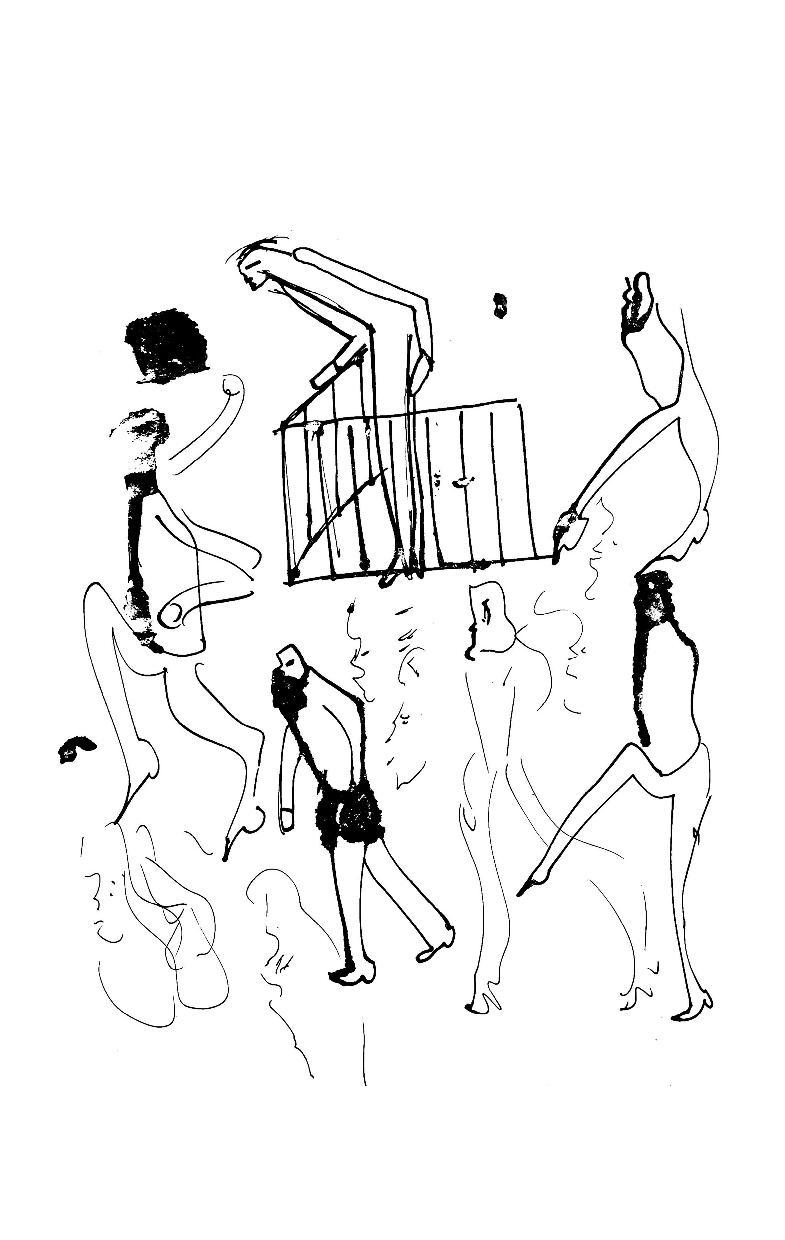
\includegraphics[width=\textwidth]{./IMAGENS/ESCOLHIDAS/IMG-07.pdf}
\end{figure}

E assim ela não se deixou dissuadir de sua decisão pela mãe que, presa de
pura inquietação, se sentindo muito insegura dentro do quarto, logo se
calou e ajudou a irmã, na medida de suas forças, a levar o guarda-roupa
para fora. Ora, em último caso Gregor ainda podia dispensar este móvel,
mas a escrivaninha, esta tinha que ficar. E as mulheres mal haviam deixado
o quarto com o guarda-roupa, contra o qual se espremiam, gemendo, quando
Gregor projetou a cabeça por baixo do canapé, para ver como daria para
interferir com prudência e o máximo de delicadeza possível. Mas, por
infelicidade, foi bem a mãe quem retornou primeiro, enquanto Grete no
cômodo ao lado se atracava ao guarda-roupa e tentava balançá-lo de um lado
para o outro, é lógico que sem conseguir tirá-lo do lugar. A mãe, porém,
não estava habituada à aparência de Gregor, poderia ter um ataque, e por
isso espavorido ele retrocedeu depressa até o fundo do canapé, entretanto
não pôde mais evitar que o lençol se movimentasse um pouco na parte da
frente. Foi o suficiente para chamar a atenção da mãe. Ela estacou, ficou
um instante imobilizada e então voltou para junto de Grete.

Apesar de Gregor repetir consigo mesmo, sucessivamente, que nada de
excepcional acontecia, era tão-só a mudança de uns poucos móveis, esse vai
e vem das mulheres, as breves exortações entre elas, os riscos dos móveis
no assoalho, isso tudo o atingia, ele logo teve de reconhecer, como se
fosse um grande tumulto, com ruídos vindo de todos os lados, e mesmo
mantendo cabeça e pernas encolhidas e o corpo colado ao chão, ele se via
forçado a admitir que logo não suportaria mais aquilo. Estavam esvaziando
seu quarto; retiravam tudo o que tinha de mais caro; o guarda-roupa, onde
guardava o arco de serra e as outras ferramentas, elas já haviam levado;
agora soltavam a escrivaninha que fora bem fixada no chão, e na qual ele
escrevera suas lições no tempo da escola de comércio, do colégio e até
mesmo do primário --- de modo que não sobrava muito tempo para que avaliasse
quão boas eram as intenções das duas mulheres, de cuja real existência
aliás ele já havia quase se esquecido, pois, de exaustas, elas agora
trabalhavam mudas, e ouviam-se apenas as passadas pesadas de seus pés.\looseness=-1

E assim, pois --- na hora em que as mulheres, já no cômodo ao lado,
apoiavam-se à escrivaninha, procurando retomar o fôlego ---, ele avançou
para fora, mudou de posição quatro vezes, calculando a direção da corrida,
sem saber ao certo o que salvar primeiro, quando notou, em destaque na
parede já de todo nua, o quadro pendurado da dona vestida puramente de
peles, rastejou rápido até lá e apertou-se contra o vidro, que o prendeu e
refrescou o calor de sua barriga. Pelo menos esse quadro, que agora Gregor
cobria por completo, com certeza ninguém levaria mais embora. Ele girou a
cabeça na direção da porta da sala, para prestar atenção nas mulheres, que
retornavam.

\textls[-5]{Elas não haviam se permitido muito tempo de descanso e logo estavam de
volta; Grete vinha com o braço ao redor da mãe e como que a arrastava. “E
agora, o que levamos?”, disse e olhou ao seu redor. Foi então que se
cruzaram, seu olhar com o de Gregor na parede. Por certo só em razão da
presença materna é que ela conservou a calma, abaixou o rosto para junto
da mãe, na tentativa de impedi-la de olhar à sua volta, e falou, não
obstante trêmula e irrefletidamente: “Vamos voltar, não é melhor a gente
descansar mais um tempinho na sala?”. Para Gregor, a intenção de Grete era
clara, ela queria garantir a segurança da mãe para depois vir varrê-lo da
parede. Pois ela que experimentasse! Ele estava unido ao seu quadro e não
o entregaria. Preferia pular na cara dela.}\looseness=-1

Mas as palavras de Grete a rigor só conseguiram sobressaltar a mãe, que
deu um passo para o lado, avistou a monstruosa mancha marrom sobre as
flores do papel de parede, gritou, com uma voz gutural e aflita, antes
mesmo de tomar consciência de que aquilo que via era Gregor: “Meu Deus,
meu Deus!”, e caiu por cima do canapé, com os braços estendidos, como se
largasse mão de tudo, e não voltou a se mexer. “Você, hein, Gregor!”,
bradou a irmã de punho erguido e com o olhar severo. Eram as primeiras
palavras diretas que lhe dirigia desde a transformação. Ela correu para o
cômodo ao lado, em busca de alguma essência com que pudesse despertar a
mãe desfalecida; Gregor também queria ajudar --- a defesa do quadro podia
ser adiada ---, mas estava tão grudado ao vidro que precisou usar da força
para se soltar; em seguida correu também até o aposento vizinho,
acreditando poder dar à irmã algum conselho, como nos velhos tempos; não
conseguiu fazer nada, porém, além de ficar imóvel atrás dela; enquanto
ainda remexia em diferentes frasquinhos, ela se virou e tomou um baita
susto; um vidro caiu no chão e se espatifou; um caco feriu Gregor no
rosto, uma substância corrosiva escorreu sobre ele; Grete, sem mais perda
de tempo, simplesmente pegou tantos frascos quanto podia carregar e
disparou com eles para junto da mãe; ao sair bateu a porta com o pé.
Gregor foi assim isolado da mãe, que por culpa dele talvez estivesse a
ponto de morrer; a porta ele não devia abrir, se não quisesse espantar a
irmã, que precisava ficar ao lado da mãe; não tinha no momento nada a
fazer, a não ser esperar; então, presa de remorsos e preocupação, ele
começou a rastejar, passando por cima de tudo, paredes, móveis, teto, e
por fim, em seu desespero, logo que todo o aposento começou a girar em
torno de si, caiu bem no centro, em cima da mesa grande.

Um breve intervalo de tempo transcorreu, Gregor continuava ali deitado,
prostrado, ao redor o silêncio, talvez isso fosse um bom sinal. Então a
campainha tocou. A mocinha, logicamente, estava trancada na cozinha e por
isso Grete teve de ir abrir. O pai estava de volta. “O que aconteceu?”,
foram suas primeiras palavras; a expressão da filha por certo lhe revelara
tudo. Grete respondeu com a voz abafada, o rosto apertado contra o peito
do pai: “Mamãe teve um desmaio, mas já está melhor. Gregor escapuliu”. “Eu
já esperava por isso”, disse o pai, “era o que eu sempre dizia, mas vocês
mulheres não quiseram me dar ouvidos.” Para Gregor ficou nítido que o pai
entendera mal o relato demasiado conciso de Grete e supunha que ele
tivesse cometido alguma brutalidade. Por isso devia agora tentar
apaziguá-lo, pois para esclarecer as coisas não havia tempo, tampouco
possibilidade. De modo que se afastou até a porta do seu quarto e ficou
bem junto dela, para que o pai, assim que entrasse pela antessala, pudesse
ver que ele tinha toda a intenção de regressar imediatamente aos seus
aposentos, e que não seria preciso tocá-lo de volta, pelo contrário,
bastava apenas abrir a porta e na mesma hora ele desapareceria.\looseness=-1

Mas o pai não estava em condições de perceber tais sutilezas; “Arrá!”, ele
gritou logo ao entrar, em um tom que parecia ao mesmo tempo satisfeito e
ameaçador. Gregor tirou a cabeça da porta e a suspendeu na direção do pai.
Na verdade nunca havia imaginado o pai assim, como se apresentava agora;
além disso, nos últimos tempos, por conta da empolgação com o rastejar,
deixara de se preocupar como antes com os acontecimentos no resto do
apartamento, e portanto deveria estar pronto para encontrar muita coisa
mudada. Apesar disso, apesar de tudo, ainda era o pai? O mesmo homem que
antigamente, nas manhãs em que Gregor saía para uma viagem de negócios,
permanecia enterrado na cama, esgotado; que nas noites de regresso o
recebia no cadeirão, de pijama; incapaz de se erguer direito, podendo
apenas levantar os braços como sinal de alegria, e que nos raros passeios
da família, em um ou outro domingo do ano e nas datas mais importantes,
entre Gregor e a mãe, que em atenção a ele andavam devagar, caminhava
sempre um pouco mais devagar ainda, embrulhado em seu sobretudo gasto,
avançando a custo com a maior atenção ao apoiar a bengala, e quando queria
falar quase sempre se detinha e obrigava os outros a se reunir a seu
redor? Agora, porém, ele estava mesmo bem empertigado; metido em um
uniforme muito justo, azul com botões dourados, igual ao usado pelos
contínuos dos bancos; sobre o alto colarinho engomado do casaco
desdobrava-se sua papada dupla; sob as sobrancelhas espessas aflorava o
brilho radiante e atento dos olhos escuros; o cabelo branco, outrora todo
espetado, fora emplastrado e repartido rigorosamente ao meio em um
penteado meticuloso e luzidio. O quepe, no qual despontava um monograma
dourado, decerto de uma casa bancária, ele jogou em cima do canapé, num
lançamento em curva que cruzou todo o cômodo, depois marchou em direção a
Gregor com a cara amarrada, as abas do casaco do uniforme postas para
trás, as mãos nos bolsos da calça. Ele próprio não sabia direito como
proceder; ainda assim, erguia os pés a uma altura fora do comum, e Gregor
se espantou com as proporções colossais do solado de suas botas. Claro que
não ficaria apenas nisso, sempre soube, desde o primeiro dia de sua nova
vida, que o pai, para lidar com ele, só considerava apropriado o máximo de
rigor. Então saiu da sua frente correndo, estacando quando o pai ficava
parado e voltando a se apressar mal o pai se mexia. Desse modo deram mais
de uma vez a volta pelo cômodo, sem que algo de decisivo acontecesse,
inclusive sem que, no geral, em consequência do lento andamento, houvesse
a aparência de uma perseguição. Em vista disso, Gregor por enquanto também
se mantinha no chão, tanto mais temendo que o pai pudesse tomar uma fuga
pelas paredes ou pelo teto como uma provocação maldosa. Contudo, foi
obrigado a reconhecer que não suportaria essas corridinhas por muito mais
tempo, porque, enquanto o pai dava um passo, ele tinha de realizar um
sem-número de movimentos. A dificuldade de respirar logo começou a
aparecer, visto que, como nos velhos tempos, também não dispunha agora de
pulmões dignos de confiança. Por isso, ao se balançar para os lados, a fim
de reunir todas as forças para a corrida, nem abria os olhos; em sua
obtusidade, não conseguia pensar em outra solução a não ser correr; e
quase já havia esquecido que podia contar com as paredes, as quais,
todavia, eram aqui obstruídas por móveis finamente talhados, cheios de
pontas e quinas --- foi quando passou raspando ao lado dele alguma coisa
que, arremessada sem força, caiu e rolou à sua frente. Era uma maçã; logo
uma segunda voou em sua direção; Gregor ficou paralisado de medo; uma nova
corrida era inútil, pois o pai estava determinado a um bombardeio. Tinha
enchido os bolsos na fruteira do aparador e, sem caprichar na pontaria por
enquanto, atirava, maçã atrás de maçã. As pequenas frutas vermelhas
rolavam pelo chão, pareciam imantadas, e batiam umas contra as outras. Uma
maçã lançada de mansinho atingiu Gregor de leve, mas ricocheteou sem
maiores danos. A que veio voando logo em seguida, ao contrário, penetrou
firme em suas costas; Gregor quis ainda se arrastar como se a dor
extraordinariamente incrível fosse passar com a mudança de posição; porém
ele se sentia como se estivesse pregado e desmoronou, em completo colapso
de todos os sentidos. Só num último relance ainda pôde ver como a porta de
seu quarto se escancarou e a mãe, à frente da irmã que gritava, entrou
depressa, sem o vestido, pois a irmã a despira após o desmaio para
permitir-lhe uma respiração mais livre, como em seguida a mãe correu ao
encontro do pai e suas anáguas desapertadas escorregaram uma após a outra
até o chão, e como ela, tropeçando nas vestes caídas, atirando-se sobre o
pai e o abraçando, em completa conjunção com ele --- mas nessa hora a visão
de Gregor já vacilava ---, cruzando as mãos em torno de seu pescoço, pediu
clemência pela vida de Gregor. 

\chapter*{}
\section{III}

\noindent{}O ferimento sério, com o qual padeceu mais de um mês --- a maçã continuou,
uma vez que ninguém se atreveu a retirar, enfiada na carne, como uma
recordação exposta ---, pareceu fazer até mesmo o pai se lembrar de que
Gregor, apesar de suas feições asquerosas e deprimentes, era um membro da
família, e não merecia ser tratado que nem um inimigo, pelo contrário, no
seu caso a lei das obrigações familiares mandava engolir a repulsa e
tolerar, nada além de tolerar.

E se então, devido ao ferimento, Gregor também havia perdido certa
mobilidade, talvez para sempre, e necessitava no momento, como um veterano
mutilado, de longos e longos minutos para cruzar seu quarto --- rastejar no
alto, nem pensar ---, agora, em troca desse sensível declínio em suas
condições, recebia uma compensação em sua opinião bastante satisfatória,
dado que à noitinha a porta da sala, que uma ou duas horas antes ele já
tratava de observar com atenção, era em geral aberta para que, deitado no
escuro do seu quarto, não visível da sala, ele pudesse ver a família
reunida na mesa iluminada e escutar suas conversas, de certo modo com o
consentimento de todos, e portanto bem diferente de antes.

Decerto não eram mais aquelas reuniões calorosas dos velhos tempos, que
nos minúsculos quartos de hotel Gregor imaginara, nunca sem uma ponta de
inveja, quando, exausto, era obrigado a se enfiar nos lençóis gelados.

Tudo agora transcorria quase sempre na maior monotonia. Depois do jantar o
pai logo pegava no sono em sua cadeira; a mãe e a irmã recomendavam
silêncio uma à outra; a mãe, bastante curvada embaixo da luz, costurava
fina roupa branca para uma loja de confecções; a irmã, que arranjara um
emprego de vendedora, aprendia taquigrafia e francês à noite, para quem
sabe mais tarde obter um cargo melhor. Às vezes o pai despertava e, sem
nem se dar conta de que estivera dormindo, dizia para a mãe: “Mas que
tanto você fica aí só costurando!”, e voltava a adormecer no instante
seguinte, enquanto mãe e irmã trocavam entre si um sorriso fatigado.

Com uma birra particular, o pai nem em casa aceitava tirar seu uniforme de
serviço; e enquanto o pijama pendia inútil no cabide ele cochilava no seu
canto completamente vestido, como se estivesse sempre a postos para o
trabalho e mesmo aqui esperasse pelas ordens do supervisor. Em
consequência disso, o uniforme, que já não era novo no começo, não parava
limpo, apesar de todo o cuidado da mãe e da irmã, e Gregor olhava várias
vezes a noite inteira para aquela roupa vistosa, com seus botões dourados
superlustrados, e a cada dia mais cheia de nódoas, com a qual o velho no
maior desconforto dormia, entretanto, bem tranquilo.

Na hora em que o relógio chegava às dez, a mãe, fingindo bronquear,
chamava o pai e em seguida tentava persuadi-lo a ir para a cama, pois ali não
era lugar de dormir e uma boa noite de sono seria imprescindível para ele,
que devia se apresentar às seis da manhã em seu emprego. Mas, com a teima
que tinha desde que estava empregado, o pai sempre insistia em permanecer
à mesa, embora invariavelmente adormecesse, e então, além de tudo, era a
maior mão-de-obra induzi-lo a trocar a cadeira pela cama. Por mais que a
mãe e a irmã o animassem com breves incentivos, ele ficava uns quinze
minutos balançando devagar a cabeça, mantinha os olhos fechados, e não se
levantava. A mãe o puxava pela manga, sussurrava palavras ternas ao pé do
seu ouvido, a irmã deixava as lições para ajudá-la, mas com o pai isso de
nada valia. Ele só afundava ainda mais na cadeira. Apenas quando as
mulheres o tomavam pelos braços é que ele entreabria os olhos, olhava
alternado para a mãe e para a irmã, fazendo questão de dizer: “Isto é que
é vida. Este é o sossego da minha velhice”. E apoiado nas duas se
levantava, com muita dificuldade, como se fosse ele mesmo o que mais lhe
pesava, deixava-se conduzir pelas mulheres até a porta, lá as dispensava e
prosseguia então sozinho, enquanto a mãe largava às pressas o estojo de
costura, a irmã a pena, para irem correndo atrás dele e continuar ajudando.

Nessa família esfalfada e moída pelo trabalho, quem teria tempo para se
ocupar com Gregor além do estritamente necessário? O orçamento doméstico
era cada vez mais apertado; a empregada já fora inclusive dispensada; uma
faxineira enorme e robusta, com uma cabeleira branca esvoaçando pela
cabeça, vinha agora pela manhã e no final da tarde para dar conta do
serviço pesado; o restante sobrava para a mãe, junto com suas muitas
obrigações de costura. Até aconteceu de diversas joias da família, que no
passado a mãe e a irmã chegaram a ostentar radiantes em recepções e
cerimônias, terem de ser vendidas, como Gregor veio a saber à noite pela
falação geral em torno do montante obtido. A maior reclamação, porém, era
sempre a de que não podiam abandonar aquele apartamento, grande demais nas
atuais circunstâncias, por não saberem como incluir Gregor na mudança. Mas
Gregor percebia muito bem que não era apenas a preocupação com ele que
impedia uma mudança, pois seria simples transportá-lo em uma caixa
apropriada, com alguns furos para a entrada de ar; o que realmente
refreava a troca de apartamento era muito mais a total falta de esperanças
da família e o pensamento de que uma desgraça tal os fustigava, como nunca
a ninguém em todo o seu círculo de parentes e conhecidos. O que o mundo
demandava aos
%Iuri:cobravam dos
pobres, eles ofereciam ao máximo,
%Iuri:cumpriam totalmente
o pai ia buscar café para
os funcionários do baixo escalão do banco, a mãe se sacrificava pela roupa
íntima de pessoas estranhas, a irmã corria de um lado para o outro do
balcão atrás das exigências dos fregueses, mas as forças da família já
estavam no limite. E a ferida aberta nas costas voltava a doer em Gregor
como na primeira vez, quando a mãe e a irmã, depois de colocarem o pai na
cama, regressavam, deixavam a ocupação de lado, aproximavam-se uma da
outra e sentavam-se já de rosto colado; quando a mãe, apontando para
o quarto de Gregor, dizia: “Fecha aquela porta, Grete”, e quando enfim
Gregor voltava à escuridão, enquanto do outro lado as mulheres misturavam
suas lágrimas ou então, sem lacrimejar, contemplavam a mesa desconsoladas.

\begin{figure}[p]
\centering
\thisfloatpagestyle{empty}
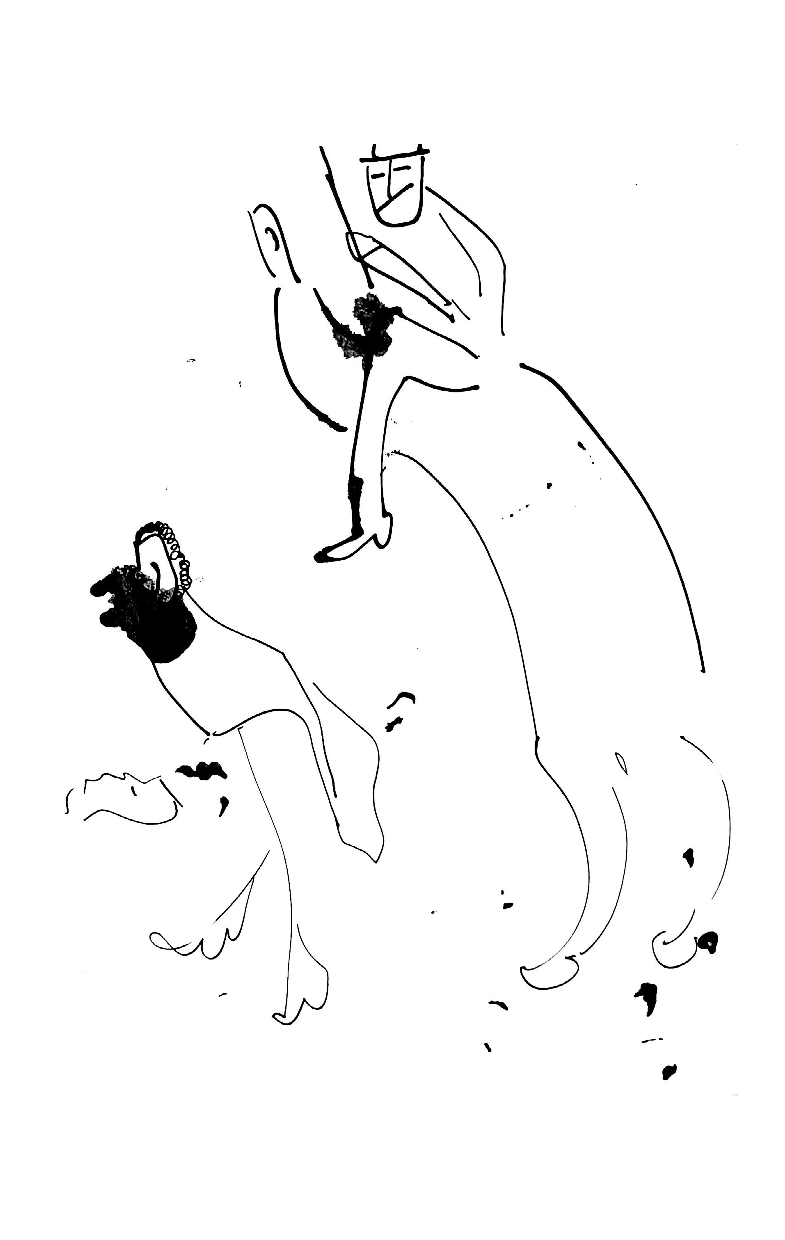
\includegraphics[width=\textwidth]{./IMAGENS/ESCOLHIDAS/IMG-09.pdf}
\end{figure}

Gregor desperdiçava as noites e os dias e já quase não dormia. Algumas
vezes pensava em retomar as rédeas dos assuntos da família, igualzinho
como antes, na próxima vez que a porta fosse aberta; em seus pensamentos
voltavam a aparecer, depois de muito tempo, o chefe e o gerente, os
balconistas e os aprendizes, o imbecil do menino de recados, dois ou três
colegas de outras lojas, uma camareira de um hotel no interior,
lembrança querida e fugaz, uma atendente de caixa de uma loja de chapéus,
a quem cortejara a sério porém de modo muito tímido --- todos eles apareciam
misturados com pessoas estranhas ou já esquecidas, só que não serviam de
ajuda a ele e à sua família, ao contrário, eram indistintamente
inapeláveis, e Gregor ficava contente quando desapareciam. Mas daí não
tinha mais nenhuma gana de se preocupar com a família, sobrevinha apenas a
raiva pelo desleixo e, apesar de não poder imaginar nada que atiçasse o
seu apetite, planejava um modo de alcançar a despensa para retirar de lá
ao menos o que lhe era devido, ainda que não estivesse com fome. A irmã
agora, de manhã e ao meio-dia, antes de sair correndo para a loja, sem nem
cogitar uma forma de fazer um agrado especial a ele, empurrava para dentro
do quarto às pressas, com o pé, algum resto de comida qualquer, que à
noitinha ela botava para fora com uma vassourada, nem reparando se a
comida por acaso havia sido provada ou --- caso mais frequente --- continuava
perfeitamente intacta. A arrumação do quarto, de que ela agora só se
ocupava à noite, não poderia ser feita de modo mais rápido. Trilhas de
sujeira se estendiam pelas paredes, em toda parte cresciam montinhos de pó
e lixo. Nas primeiras vezes, assim que a irmã entrava, Gregor se
posicionava de maneira a deixar patente a sua insatisfação. Mas poderia ficar ali parado uma
semana, sem que a irmã se emendasse; ela enxergava a imundície tanto
quanto ele, porém estava determinada a ignorá-la. Ademais, com uma
suscetibilidade há pouco tempo adquirida, que a propósito contaminara toda
a família, ela zelava para que a arrumação do quarto de Gregor ficasse
exclusivamente por sua conta. Uma vez a mãe submeteu o quarto a uma faxina
geral, tarefa somente possível com o emprego de várias tinas de
água --- a umidade em excesso, no fim, também fez mal a Gregor e ele foi
deitar em cima do canapé, meio grogue, amargurado e incapaz de se mover ---,
mas o castigo da mãe não tardou a chegar. Pois à noite a irmã, mal notara
a mudança no quarto, voltou correndo para a sala, ofendidíssima, e, não
obstante o gesto de súplica das mãos erguidas da mãe, irrompeu numa crise
de choro que os pais --- o pai naturalmente acordou de um pulo de sua
cadeira --- a princípio observaram aturdidos e sem ação; até que também se
condoeram; o pai repreendia a mãe à direita, por não ter deixado à irmã a
limpeza do quarto de Gregor; à esquerda, por outro lado, berrava com a
irmã, exigindo que ela nunca mais limpasse aquele quarto; enquanto a mãe
tentava levar para a cama o pai, que ficara fora de si nesse alvoroço, a
irmã, sacudida pelos soluços, martelava a mesa com seus punhos pequenos; e
Gregor silvava alto de raiva, porque ninguém havia se lembrado de fechar a
porta e poupá-lo da cena e de toda aquela barulheira.

Mas mesmo se a irmã, exaurida por sua atividade profissional, estivesse
cheia de cuidar dele como cuidava antes, a mãe não teria de modo algum
obrigação de rendê-la e Gregor ainda assim não precisava ficar ao
desamparo. Pois agora tinham a faxineira. Essa velha viúva, que em sua
longa vida devia ter superado as piores situações com a ajuda de sua
notável robustez, não nutria a rigor nenhuma aversão por Gregor. Não sendo
de modo algum curiosa, havia uma vez por acaso aberto a porta do quarto
dele, que pego de surpresa começou a correr de um lado para outro, embora
ninguém o perseguisse, e ao avistá-lo ela continuou de pé onde estava, as
mãos cruzadas no peito, admirada. Desde então, não passava um dia sem
entreabrir a porta, de manhã e no final da tarde, para espiar Gregor um
minutinho. No começo, ela também o chamava com palavras que devia julgar
simpáticas, tais como “Vem cá, bichão!” ou “Cadê o velho besourão?!”.
Gregor não atendia a esses chamados, ficava mais é quieto no seu canto,
como se a porta nem tivesse sido aberta. Se ao menos fosse ordenado a essa
faxineira que, em vez de satisfazer seus caprichos indo perturbá-lo para
nada, limpasse seu quarto todos os dias! Certa ocasião, de manhã cedinho ---
uma chuva pesada golpeava a vidraça, talvez já um sinal anunciando a
primavera ---, logo que a faxineira veio de novo com aquele jeito de falar,
Gregor ficou irritado de tal modo que se virou para ela, é certo que num
passo lento e debilitado, como se fosse partir para o ataque. A faxineira,
porém, em vez de se intimidar, simplesmente tomou uma cadeira que
encontrou ao lado da porta, ergueu-a bem no alto e, do modo como ficou
parada lá com a bocona escancarada, era clara sua intenção de só fechá-la
quando a cadeira em suas mãos tivesse baixado nas costas dele. “Não vai
avançar mais?”, ela perguntou, ao vê-lo retroceder, e pôs de volta
tranquila a cadeira em seu lugar.

Gregor já não comia quase nada. Só quando por acaso topava com a comida
disponível é que abocanhava de brincadeira uma pequena porção, que
mantinha na boca horas a fio e depois cuspia fora, na maior parte das
vezes. A princípio pensou que era a tristeza com o estado de seu quarto
que o impedia de comer, mas foi justo com as mudanças do quarto que ele se
conformou mais depressa. Coisas que não podiam ser alojadas em outra parte
eram jogadas lá dentro, e agora havia muitas dessas coisas, dado que um
quarto do apartamento havia sido alugado para três inquilinos. Esses
senhores muito sérios --- todos os três usavam barba, como Gregor averiguou
certa vez por uma fresta da porta --- eram cheios de escrúpulos quanto à
ordem, não apenas no quarto que ocupavam, mas também, já que agora estavam
hospedados ali, em toda a casa, particularmente na cozinha. Não toleravam
trastes inúteis, muito menos sujos. Além disso haviam trazido consigo, em
grande parte, seus próprios móveis e objetos de decoração. Por esse motivo
muitas coisas se tornaram supérfluas, coisas que na verdade não eram
vendáveis, mas que também não se queria jogar fora. Todas elas rumaram
para o quarto de Gregor. Mesmo destino da caixa de cinzas e do cesto de
lixo da cozinha. Bastava que algo não tivesse utilidade no momento para
que a faxineira, sempre com muita pressa, simplesmente o atirasse para
dentro do quarto de Gregor; na maioria das vezes, por sorte, Gregor via só
o objeto em questão e a mão que o segurava. Pode ser que a faxineira
tivesse a intenção, havendo tempo e oportunidade, de pegar as coisas de
volta ou então de jogar tudo fora de uma vez, mas na prática elas ficavam
por lá, largadas no mesmo local onde haviam sido atiradas, a não ser
quando Gregor se retorcia no meio da tralha e começava a deslocá-las, no
começo forçado, porque já não sobrava espaço livre para rastejar, mas
depois com uma alegria crescente, embora, ao final dessas excursões, morto
de cansaço e mágoa, ficasse horas sem poder se movimentar de novo.

Como os inquilinos às vezes jantavam em casa, na sala, que era de uso
comum, a porta que dava para lá permanecia fechada algumas noites, mas
Gregor abdicava de sua abertura sem dificuldade, já tendo inclusive
deixado de aproveitá-la em várias ocasiões em que fora franqueada,
preferindo ficar encolhido, sem que a família percebesse, no canto mais
escuro do seu quarto. Uma vez, porém, a faxineira deixou essa porta um
tanto entreaberta, e assim ela ficou, mesmo quando os inquilinos entraram
à noite e a luz foi acesa. Eles foram se sentar à ponta da mesa, onde
antigamente o pai, a mãe e Gregor comiam, desdobraram os guardanapos e
empunharam garfo e faca. Na mesma hora a mãe apareceu na porta com uma
travessa de carne e bem atrás dela a irmã com outra travessa transbordando
de batatas. A comida fervia numa nuvem de vapor. Os inquilinos se curvaram
sobre as travessas colocadas à sua frente, como se quisessem dar uma
conferida antes de comer, e de fato o que estava sentado no meio, e
parecia ter mais autoridade que os outros dois, deu um talho na carne
ainda na travessa, averiguando de modo ostensivo se estava tenra o
suficiente e se não era o caso de devolvê-la à cozinha. Ele ficou
satisfeito, e a mãe e a irmã, que observavam apreensivas, puderam suspirar
com um sorriso de alívio.

A família mesmo foi comer na cozinha. Apesar disso, antes de ir para lá o
pai veio até a sala e, com uma única mesura, o quepe na mão, deu a volta
em torno da mesa. Os inquilinos levantaram-se juntos e murmuraram de má
vontade qualquer coisa lá com suas barbas. Quando então ficaram a sós,
comeram quase que em total silêncio. Gregor achou estranho que, de todos
os diversos ruídos que acompanham uma refeição, o mais perceptível fosse o
som de dentes mastigando, como se com isso devesse ser mostrado a ele que
para comer eram necessários dentes, e que com mandíbulas banguelas, mesmo
as mais bonitas, não se obtém sucesso. “Eu tenho sim vontade de comer”,
Gregor disse a si mesmo, muito preocupado, “só que não essas
coisas. Como comem esses inquilinos, e eu aqui definhando!”

Bem naquela noite --- Gregor não se lembrava de tê-lo escutado em todo
aquele tempo --- veio da cozinha o som do violino. Os inquilinos já haviam
terminado sua refeição noturna, o do meio desdobrou um jornal, deu aos
outros dois uma folha cada, e agora eles liam recostados e fumavam. Quando
o violino começou a soar, tiveram a atenção despertada, ergueram-se e
foram na ponta dos pés até a porta da antessala, onde ficaram parados, um
espremido contra o outro. Devem ter sido ouvidos da cozinha, pois o pai
gritou de lá: “A música não agrada aos senhores? Ela pode parar agora
mesmo”. “Pelo contrário”, disse o senhor do meio, “a menina não quer vir
até aqui tocar na sala, que é muito mais cômodo e agradável?” “Oh, como
não!”, gritou o pai, como se fosse ele o violinista. Os senhores voltaram
para a sala e esperaram. Logo chegou o pai com a estante, a mãe com a
partitura e a irmã com o violino. A irmã calmamente ajeitou tudo para
tocar; os pais, que nunca antes haviam alugado quartos e por isso se
excediam na cortesia com os inquilinos, nem se atreveram a sentar nas
próprias cadeiras; o pai encostou na porta, a mão direita enfiada entre
dois botões do casaco abotoado; a mãe, porém, aceitou a cadeira oferecida
por um dos senhores e, como não a moveu do local onde ele por acaso a
colocara, acabou sentando afastada.

A irmã começou a tocar; pai e mãe, cada qual do seu lado, seguiam atentos
os movimentos das mãos dela. Gregor, atraído pela música, arriscou-se um
pouco mais à frente e logo estava com a cabeça na sala. Já nem se admirava
de que, nos últimos tempos, demonstrasse tão pouca consideração pelos
outros; antigamente esse tipo de respeito era para ele um motivo de
orgulho. E na verdade teria justo agora muito mais razões para não
aparecer, porque, por causa da poeira que tomava conta de seu quarto e que
ao menor movimento se espalhava no ar, ele também vivia coberto de pó;
arrastava consigo fiapos, pelos, restos grudados dos lados e nas costas;
sua apatia diante de tudo era muito grande para que se desse ao trabalho
de deitar de costas, como fazia antes várias vezes ao dia, e se esfregar
no tapete. E mesmo nesse estado ele não teve o menor pudor de invadir um
pedaço do piso imaculado da sala.

Em todo caso ninguém nem reparava nele. A família estava bastante absorta
pelo som do violino; ao contrário dos inquilinos, que a princípio, as mãos
nos bolsos das calças, haviam se posicionado bem atrás da estante, muito
próximos da irmã, de modo a que pudessem todos os três acompanhar as
notas, o que com certeza devia atrapalhá-la, mas logo, conversando a meia
voz, as cabeças abaixadas, se afastaram para junto da janela, onde
permaneceram, observados pelo olhar apreensivo pai. Essa atitude realmente
tinha a aparência mais do que clara de que eles haviam sido frustrados em
sua intenção de ouvir ao violino uma música bela ou animada, que estavam
fartos daquela apresentação e que apenas por educação ainda admitiam ter
sua paz perturbada. Sobretudo o modo como todos eles sopravam para o alto
a fumaça de seus charutos, pelo nariz e pela boca, dava a entender um alto
grau de irritação. E todavia a irmã tocava tão bonito. Seu rosto pendia
para o lado, seus olhos aguçados e tristes acompanhavam as linhas da
pauta. Gregor rastejou outro tanto adiante e manteve a cabeça bem junto ao
chão, para assim, quem sabe, poder interceptar o olhar dela. Era por ser
um animal que a música o atraía tanto? A ele parecia como se tivesse à sua
frente o caminho para o ansiado alimento desconhecido. Estava decidido a
avançar até a irmã, puxá-la pela saia, e desse modo fazê-la entender que
ela poderia com prazer vir ao quarto dele com o violino, pois ninguém aqui
valorizava a música como ele quisera valorizar. Queria então não mais
deixá-la sair do quarto, pelo menos não enquanto estivesse vivo; sua
figura medonha pela primeira vez lhe seria útil; queria estar ao mesmo
tempo diante de todas as portas, bufando feito uma fera contra os
opressores; a irmã, porém, não devia ficar com ele à força, e sim por
vontade própria; ela iria se sentar ao lado dele no canapé, inclinar o
ouvido em sua direção, e ele queria nesse momento confidenciar a ela que
tivera o firme propósito de mandá-la para o conservatório, e que, se nesse
meio tempo a desgraça não houvesse ocorrido, no último Natal --- o Natal já
tinha passado, aliás? ---, ele teria anunciado o fato a todos, sem se
importar com qualquer tipo de objeção. Depois dessa explicação, a irmã
iria desatar num choro comovido, e Gregor, erguendo-se até altura do ombro
dela, lhe daria um beijo no pescoço que, desde que entrara na loja, ela
trazia sem fita nem cordão.

“Senhor Samsa!”, gritou para o pai o senhor do meio e, sem desperdiçar
mais palavras, apontou o dedo indicador na direção de Gregor, que avançava
devagar. O violino ficou mudo, o inquilino intermediário, num único
movimento de cabeça, sorriu para seus amigos e então voltou a olhar para
Gregor. Ao pai pareceu que o mais urgente era, em vez de tocar Gregor,
primeiro acalmar os inquilinos, embora estes não estivessem nada nervosos
e Gregor parecesse animá-los bem mais do que a música do violino. Ele
correu para o lado deles e com os braços abertos tentou conduzi-los a seus
aposentos e ao mesmo tempo bloquear com o corpo a visão de Gregor. Aí eles
de fato se zangaram um pouco, não dava para saber se com o comportamento
do pai ou se com a descoberta que acabavam de fazer, de que, sem que
soubessem, tinham como vizinho de quarto um tipo igual a Gregor. Exigiram
explicações do pai, ergueram como ele os braços, beliscaram as barbas com
impaciência e só a custo foram aos poucos recuando aos seus aposentos.
Enquanto isso a irmã conseguiu sair do estado de alheamento em que havia
caído com a interrupção súbita da música, depois de sustentar mais um
instante o violino e o arco nas mãos que pendiam frouxas, e em seguida
olhar para a partitura como se ainda estivesse tocando, conseguiu se recompor
num átimo, colocou o instrumento no colo da mãe, que com dificuldades
respiratórias e intensa atividade pulmonar seguia sentada em sua cadeira,
e foi correndo para o quarto ao lado, do qual, empurrados pelo pai, os
inquilinos se aproximavam agora mais depressa. Era de ver como, sob as
mãos treinadas da irmã, cobertas e travesseiros voavam pelo ar e pousavam
já dispostos direitinho nas camas. Ainda antes dos senhores chegarem à
entrada do quarto, ela já dera conta da arrumação e saíra de fininho. O
pai pareceu de novo tomado por sua teimosia, de uma tal forma que olvidou
todo o respeito a que estava obrigado perante seus locatários. Ele só
insistia e voltava a empurrar, até que, na porta do quarto, o senhor do
meio bateu com força o pé no chão, e desse modo conseguiu deter o pai.
“Declaro para todos os fins”, ele falou, ergueu a mão e dirigiu o olhar
também para a mãe e a irmã, “que, em vista das condições repugnantes em
vigor nesta casa e nesta família” --- nesse ponto ele, decidido, deu uma
breve cusparada no chão ---, “dou por cancelada minha locação. É evidente
que não pagarei o mínimo que seja, nem pelos dias em que aqui estive
hospedado, muito pelo contrário, ainda hei de ponderar se não apresento
contra o senhor uma queixa formal que --- o senhor pode ter certeza --- seria
bem fácil de justificar.” Ele se calou e olhou fixo à sua frente, como se
esperasse alguma coisa. Ato contínuo, seus amigos vieram com as palavras:
“Nós também cancelamos a nossa”. A seguir ele agarrou a maçaneta e fechou
ruidosamente a porta.

\begin{figure}[p]
\centering
\thisfloatpagestyle{empty}
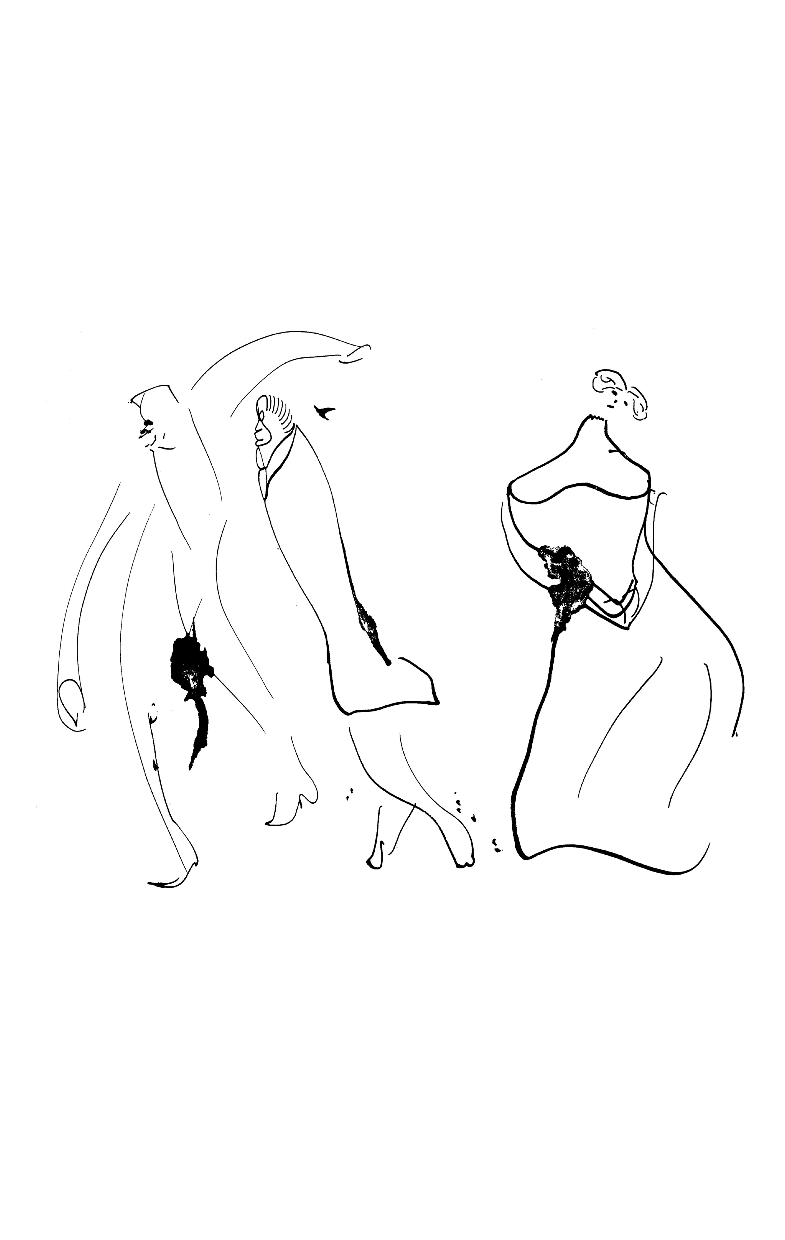
\includegraphics[width=\textwidth]{./IMAGENS/ESCOLHIDAS/IMG-11.pdf}
\end{figure}

O pai, tateando com as mãos, voltou cambaleando até sua cadeira e ali
desabou; dava a impressão de que se recostava para sua soneca noturna
cotidiana, mas os intensos meneios da cabeça, que parecia solta, mostravam
que de modo nenhum estava dormindo. Gregor ficou esse tempo todo quieto,
deitado no mesmo lugar em que fora surpreendido pelos inquilinos. O
desapontamento com o insucesso de seus planos mas talvez também a fraqueza
provocada pela fome extrema impossibilitavam que se movimentasse. Com uma
certa garantia, temia já para o instante seguinte a tempestade coletiva a
desabar em cima dele, e esperava. Não o perturbou nem mesmo o violino na
hora em que caiu do colo da mãe, depois de escorregar de seus dedos
trêmulos, e produziu um estampido retumbante.

“Meus pais”, falou a irmã e bateu a mão na mesa à guisa de introdução,
“não dá para continuar assim. Se vocês por acaso não enxergam desse jeito,
eu enxergo. Não quero usar o nome do meu irmão com esse monstro, então só
digo uma coisa: temos que nos livrar disso. Tentamos o que era humanamente
possível para criá-lo e suportá-lo, acho que ninguém tem o menor direito
de nos condenar.”

“Ela está coberta de razão”, o pai disse consigo mesmo. A mãe, que ainda
não conseguia respirar normalmente, levou a mão à boca e começou a tossir
para dentro, com uma expressão de insanidade no olhar.

A irmã correu para junto da mãe e amparou-lhe a testa. O pai, levado pelas
palavras da irmã, pareceu ter encontrado ideias mais precisas,
endireitou-se na cadeira, brincou com o quepe do uniforme em meio aos
pratos largados sobre a mesa, ainda do jantar dos inquilinos, e olhou uma
vez ou outra para Gregor, que permanecia quieto.

“Temos que dar um jeito de nos livrar dessa coisa”, a irmã falou, agora
exclusivamente para o pai, pois a mãe, com a tosse, não escutava nada,
“isso vai acabar matando vocês dois, só estou vendo a hora. Quem é
obrigado a trabalhar tanto quanto nós três não pode ainda ter que aturar
em casa esse tormento sem fim. Eu já não suporto mais.” E rompeu num choro
tão forte que suas lágrimas espirraram no rosto da mãe, que as enxugou com
movimentos mecânicos da mão.

“Filha”, falou o pai morrendo de pena e exagerando na compreensão, “mas o
que vamos fazer?”

A irmã apenas deu de ombros como sinal da sensação de impotência que a
acometera enquanto chorava, o que contrastava com sua segurança de antes.

“Se ele pudesse nos entender”, disse o pai com ar interrogativo; a irmã em
meio ao choro sacudiu a mão com veemência em sinal de que isso estava fora
de cogitação.

“Se ele pudesse nos entender”, repetiu o pai e fechou os olhos, para
assimilar a convicção da irmã quanto à impossibilidade do fato, “então
quem sabe fosse possível um acordo com ele. Mas assim ---”

“Que vá embora”, a irmã gritou, “é o único jeito, pai. Basta se livrar do
pensamento de que é o Gregor. Ter acreditado nisso durante tanto tempo,
essa no fundo é a nossa desgraça. Mas como essa coisa pode ser o Gregor?
Se fosse o Gregor, já teria entendido há muito tempo que é impossível a
convivência das pessoas com um bicho desses, e teria partido por vontade
própria. Então não haveria mais irmão, mas podíamos seguir tocando a vida
e preservar sua memória. Mas assim, fica esse bicho nos seguindo, expulsa
os inquilinos, com certeza quer tomar o apartamento e nos deixar dormindo
na rua. Olha aí, pai”, ela gritou de repente, “lá vem ele de novo!” E, num
pânico de todo incompreensível para Gregor, a irmã deixou até a mãe de
lado, chegou mesmo a empurrar sua cadeira, como se preferisse sacrificar a
mãe a ficar perto dele, e correu atrás do pai que também se levantou,
provocado única e exclusivamente pelo comportamento dela, e posicionou os
braços a meia altura à sua frente, na tentativa de protegê-la.

Mas Gregor não pretendia de modo algum amedrontar quem quer que fosse,
muito menos a irmã. Ele havia tão-só começado a se virar para regressar ao
seu quarto, o que em todo caso seria muito chamativo, dado que, devido às
suas condições lastimáveis, era difícil fazer a volta e ele precisava ajudar com a cabeça que por causa disso diversas vezes levantava e
batia contra o chão. Parou um pouco e olhou ao seu redor. Parece que
reconheciam sua boa intenção; tinha sido só um susto passageiro. Agora
todos o observavam calados e entristecidos. A mãe largada em sua cadeira,
as pernas estendidas uma por cima da outra, os olhos quase se fechando de
fadiga; o pai e a irmã sentados lado a lado, ela apoiando a mão atrás do
pescoço dele.

“Agora talvez me deixem completar a volta”, Gregor pensou e retomou sua
ocupação. Não conseguia evitar o ruído de sua respiração ofegante do
esforço e era obrigado a fazer uma pausa a todo momento. No mais, não era
pressionado por ninguém, havia sido deixado por sua própria conta. Depois
de completar a volta ele deu início ao retorno em linha reta. Ficou
admirado com a grande distância que o separava de seu quarto, e não
entendia como, com a sua fraqueza, tinha ainda há pouco, quase sem
perceber, percorrido o mesmo caminho. O tempo todo concentrado apenas em
rastejar depressa, ele mal reparava que não era incomodado por nenhuma
palavra, nenhum grito de sua família. Só depois de chegar à porta é que
ele virou a cabeça, não muito porque na hora sentiu um torcicolo, em todo
caso ainda viu que atrás de si nada havia mudado, apenas a irmã se
levantara. Seu último olhar avistou de relance a mãe, a essa altura já
totalmente adormecida.

Mal acabara de entrar no quarto e a porta foi fechada às pressas, com o
trinco e à chave. Gregor levou um susto tão grande com o barulho
inesperado às suas costas que suas perninhas vacilaram. Era a irmã que
tinha toda essa pressa. Já estava lá levantada só esperando, avançou então
saltitando na ponta dos pés, Gregor nem a ouviu se aproximar, e ao girar a
chave na fechadura ela gritou para os pais: “Até que enfim!”.

“E agora?”, perguntou-se Gregor e olhou a escuridão ao seu redor. Logo
veio a descobrir que não conseguia se mexer de jeito nenhum. Não ficou
surpreso, antes lhe parecia pouco natural que até então tivesse podido
andar de verdade com aquelas perninhas finas. De resto ele estava
relativamente bem. É certo que tinha dores por todo o corpo, mas para ele
era como se elas fossem ficando mais e mais fracas e estivessem a ponto de
sumir de uma vez por todas. Já mal sentia a maçã podre em suas costas e a
inflamação que a circundava, ambas cobertas por uma fina camada de poeira.
Lembrou-se de sua família com intensa ternura e amor. Sua posição a
respeito da necessidade de seu desaparecimento era na medida do possível
ainda mais convicta do que a da irmã. Ficou nesse estado meditabundo,
vazio e tranquilo, até que as três horas da manhã soaram no relógio da
torre. Ainda presenciou o despontar da claridade matutina do lado de fora
da janela. Então, independente de sua vontade, sua cabeça pendeu toda para
baixo e suas narículas expeliram sem força seu último suspiro.

Quando, de manhã cedo, a faxineira veio --- sempre afobada e com muita
energia, apesar de já lhe ter sido pedido várias vezes que o evitasse, ela
batia todas as portas de uma tal maneira que com a sua chegada já não era
mais possível dormir sossegado em nenhum cômodo do apartamento ---, a
princípio não achou nada de novo em sua habitual visitinha a Gregor.
Pensou que ele estivesse ali deitado imóvel de propósito, bancando o
ofendido; ela o julgava capaz de compreender tudo. Como por acaso estava
com a comprida vassoura nas mãos, tentou fazer cócegas nele ali mesmo da
porta. Quando isso também não resultou em nada, ela ficou brava e cutucou
um pouco mais fundo, e só após empurrá-lo de seu lugar sem encontrar
nenhuma resistência é que procurou ver melhor. Tão logo reconheceu a
realidade dos fatos, arregalou os olhos, soltou um assobio, mas não se
conteve muito tempo, e sim foi logo escancarar a porta do quarto dos pais,
gritando bem alto para dentro da escuridão: “Venham dar uma olhada, ele
bateu as botas; está lá, abotoou de vez o paletó!”.

Marido e mulher estavam sentados na cama de casal e tiveram primeiro que
se recuperar do susto com a faxineira, antes de virem a compreender o que
ela anunciava. Mas então, cada qual pelo seu lado, o senhor e a senhora
Samsa saíram depressa da cama, o senhor Samsa jogou a coberta por cima dos
ombros, a senhora Samsa apareceu só de camisola; assim entraram no quarto
de Gregor. Entrementes, fora igualmente aberta a porta da sala, onde Grete
dormia desde a chegada dos inquilinos; ela estava vestida dos pés à
cabeça, como se nem tivesse dormido, seu rosto pálido parecia demonstrar a
mesma coisa. “Morto?”, falou a senhora Samsa e olhou para a faxineira,
esperando uma resposta, embora pudesse confirmar por si só ou até
reconhecer o fato sem confirmação nenhuma. “É o que eu acho”, disse a
faxineira e como prova empurrou com a vassoura o cadáver de Gregor um bom
pedaço para o lado. A senhora Samsa reagiu como se fosse tentar parar a
vassoura, mas não fez nada. “Bom”, falou o senhor Samsa, “agora podemos
agradecer a Deus.” Ele fez o sinal da cruz, e as três mulheres seguiram o
seu exemplo. Grete, que não tirava os olhos do cadáver, disse: “Vejam como
ele estava magro. Já fazia um bom tempo que não comia nada. A comida
voltava do jeito que ia”. De fato o corpo de Gregor estava bem achatado e
seco, e só agora é que reparavam nisso, quando ele não mais se erguia
sobre suas perninhas e também nenhuma outra coisa distraía a atenção.

“Vamos, Grete, entra um pouquinho com a gente”, disse a senhora Samsa com
um sorriso tristonho, e Grete, não sem voltar a olhar o cadáver mais uma
vez, entrou atrás dos pais no quarto do casal. A faxineira fechou a porta
e abriu toda a janela. Embora ainda fosse cedo, uma certa tepidez
misturava-se ao ar fresco da manhã. Já era sem dúvida o final de março.

Os três inquilinos saíram de seu quarto e atônitos procuraram com os olhos
pelo café da manhã; haviam sido esquecidos. “Cadê o café da manhã?”, o
senhor do meio perguntou mal-humorado à faxineira. Esta porém pôs o
indicador na frente da boca e a seguir, em silêncio, fez apressada um
sinal indicando aos inquilinos que por favor passassem ao quarto de
Gregor. Eles passaram e ficaram lá de pé, as mãos nos bolsos de seus
paletós curtos e um tanto gastos, no quarto já totalmente iluminado, em
torno do cadáver.

Foi quando a porta do quarto dos pais se abriu, e o senhor Samsa apareceu
de uniforme, sua esposa apoiada em um braço, sua filha no outro. Todos com
cara de quem tinha chorado um pouco; Grete vez por outra pressionava o
rosto no braço do pai.

\begin{figure}[p]
\centering
\thisfloatpagestyle{empty}
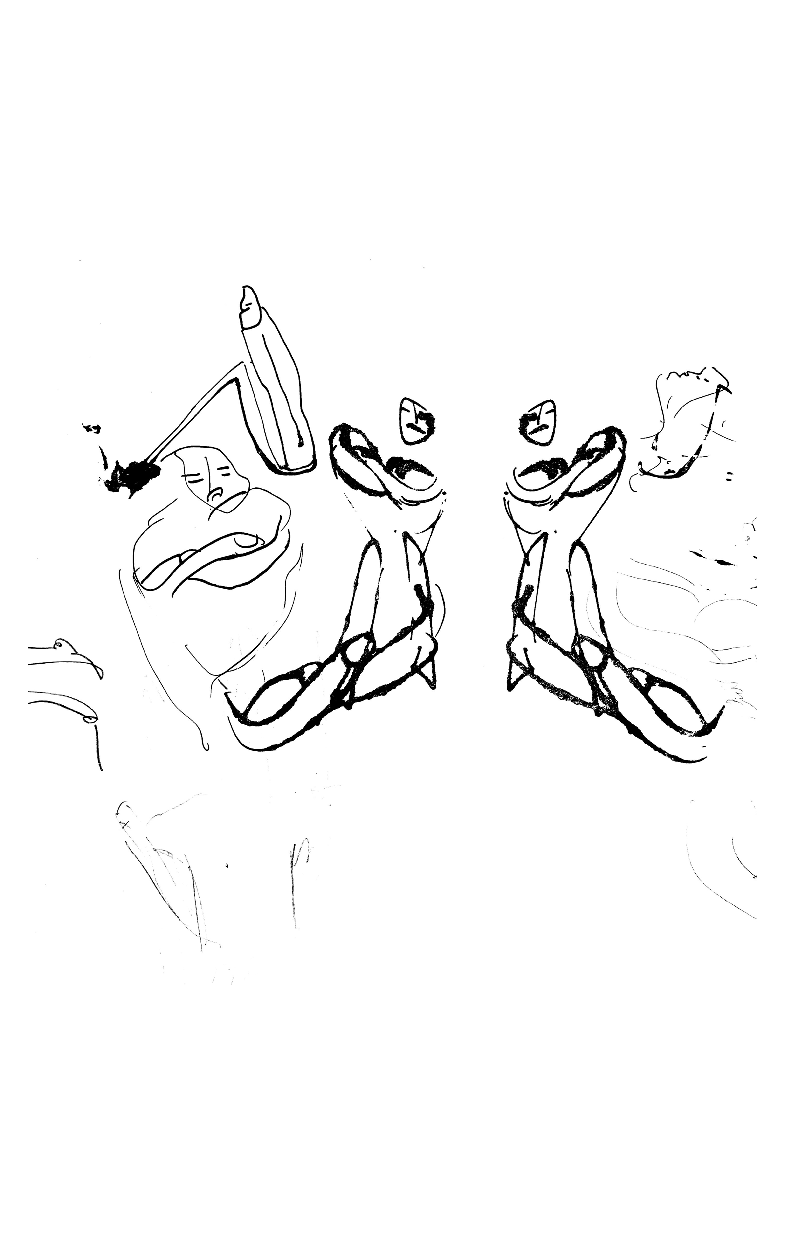
\includegraphics[width=\textwidth]{./IMAGENS/ESCOLHIDAS/IMG-12.pdf}
\end{figure}

“Saiam agora mesmo da minha casa!”, disse o senhor Samsa e apontou para a
porta, sem soltar as mulheres. “O que significa isso?”, disse o senhor do
meio um pouco espantado e com um sorriso amarelo. Os outros dois mantinham
as mãos para trás e esfregavam uma na outra, na alegre expectativa de uma
grande peleja, cujo resultado entretanto deveria ser favorável a eles.
“Significa exatamente o que acabo de dizer”, respondeu o senhor Samsa e
avançou em coluna com suas duas companheiras para cima do inquilino. Este
a princípio ficou parado onde estava e olhou para baixo, como se as coisas
em sua cabeça assumissem uma nova configuração. “Se é assim, nós vamos
embora”, acabou dizendo e ergueu o olhar para o senhor Samsa, como se, num
acesso repentino de humildade, tivesse de pedir permissão até mesmo para
uma decisão dessas. O senhor Samsa, de olhos bem abertos, limitou-se a
acenar brevemente com a cabeça uma e outra vez. O inquilino, com efeito,
em obediência a isso, de imediato se dirigiu a passos largos para a
antessala; seus dois amigos já estavam de sobreaviso há algum tempo, com
as mãos bem quietinhas, e em dois pulos seguiram no seu encalço, como se
temendo que o senhor Samsa pudesse alcançar a antessala antes deles e
perturbar o vínculo que mantinham com o líder. Na antessala, todos os três
pegaram seus chapéus no cabideiro, retiraram suas bengalas do
porta-bengalas, curvaram-se num cumprimento mudo e deixaram o apartamento.
Com uma desconfiança que se revelou infundada, o senhor Samsa saiu com as
duas mulheres no corredor; debruçados no corrimão, ficaram observando como
os três senhores, é certo que devagar, porém de modo ininterrupto, desciam
a comprida escadaria, a cada andar desapareciam em uma determinada curva
da escada e alguns segundos depois voltavam a aparecer; quanto mais para
baixo iam, mais se perdia o interesse da família Samsa por eles, e quando
um empregado do açougue surgiu, cruzou com eles e, todo aprumado e
orgulhoso, continuou subindo com um pacote em cima da cabeça, logo o
senhor Samsa abandonou o corrimão ao lado das mulheres e todos, parecendo
aliviados, regressaram ao apartamento.

Decidiram aproveitar o dia para descansar e passear; não só tinham direito
a essa folga no trabalho, ela também lhes era mais do que necessária. E
assim foram se sentar à mesa e redigir três justificativas, o senhor Samsa
à direção do banco, a senhora Samsa ao dono da loja e Grete ao seu patrão.
Estavam escrevendo quando a faxineira veio dizer que já ia, pois havia
acabado o serviço da manhã. Ocupados com a escrita, os três a princípio
apenas acenaram com a cabeça, sem erguer os olhos, só quando notaram que a
faxineira demorava a sair é que resolveram olhar para ela, contrariados.
“O que foi?”, perguntou o senhor Samsa. A faxineira estava parada na
porta, sorridente, como se tivesse uma notícia muito boa para dar à
família, porém só faria isso se lhe fosse solicitado com alguma
insistência. Fincada quase reta em seu chapéu, a pequena pluma de
avestruz, que tanto irritava o senhor Samsa durante todo o expediente
dela, oscilava de leve em todas as direções. “Mas o que a senhora quer
afinal?”, perguntou a senhora Samsa, por quem a faxineira ainda nutria o
máximo de respeito. “Está bem”, respondeu a faxineira e não conseguiu
falar muito mais por causa da risada amistosa, “o negócio aí do lado, a
senhora não vai precisar se incomodar em pôr para fora. Está tudo
resolvido.” A senhora Samsa e Grete inclinaram-se sobre o papel, dando a
entender que queriam continuar escrevendo; o senhor Samsa, ao perceber que
a faxineira agora queria começar a descrever tudo em detalhes, cortou a
conversa levantando a mão de maneira decidida. Vendo que não tinha licença
para contar, lembrou que estava com pressa, falou bem alto, visivelmente
ofendida: “Passar bem”, deu meia volta enfurecida e saiu do apartamento
debaixo de um assombroso bater de portas.

“Hoje mesmo ela vai ser despedida”, disse o senhor Samsa, sem porém obter
resposta, nem de sua esposa, nem de sua filha, pois a faxineira parecia
ter perturbado o sossego que acabavam de alcançar. Elas se levantaram,
foram até a janela e lá ficaram, abraçadas uma à outra. O senhor Samsa
virou-se para elas sem sair de sua cadeira e ficou observando quieto um
momento. Então reclamou: “Ora, venham até aqui. Deixem em paz as coisas
passadas. E tenham um pouco de consideração por mim”. As mulheres o
obedeceram no ato, voltaram depressa para ele, fizeram-lhe festinhas, e
logo terminaram de escrever suas justificativas.

Então todos os três saíram juntos do apartamento, o que já não faziam há
meses, e seguiram de bonde rumo aos espaços abertos nos arredores da
cidade. O vagão em que se sentaram a sós reluzia com o brilho quente do
sol. Comodamente reclinados em seus assentos, eles avaliaram suas
perspectivas de futuro e acharam que, examinando mais de perto, elas não
seriam assim tão ruins, pois todos os três empregos eram, embora não
tivessem informações muito precisas um do outro a esse respeito,
sobremaneira oportunos e, a longo prazo, bastante promissores. A principal
melhoria em sua situação no momento deveria advir sem muita dificuldade
com a mudança de residência; queriam agora alugar um apartamento menor e
mais barato, porém mais bem localizado e acima de tudo mais prático do que
o atual, que havia sido ainda uma escolha de Gregor. Enquanto conversavam
sobre essas coisas, o senhor e a senhora Samsa, admirados com a vivacidade
crescente da filha, notaram praticamente no mesmo instante como ela nos
últimos tempos, apesar de todo o sofrimento responsável pela palidez em
suas faces, desabrochara e era agora uma moça bonita e cheia de viço. Cada
vez mais calados e entendendo-se quase que por instinto só com a troca de
olhares, pensaram que já era tempo de arranjar um bom marido para ela. E
foi para eles como que uma confirmação de seus novos sonhos e belos
projetos quando, no final da viagem, a filha se levantou primeiro e
espreguiçou seu corpo jovem.